\documentclass[11pt,twoside,openany]{book}

\usepackage[letterpaper,left=.87in,right=.87in,top=.84in,bottom=.84in,headheight=20pt,headsep=16pt,footskip=25pt]{geometry}
\usepackage[T1]{fontenc}
\usepackage{lmodern,anyfontsize}
\usepackage[scaled=.94]{helvet}
\usepackage[utf8]{inputenc}
\usepackage{amsmath,amssymb,amsthm,mathtools,bm}
\usepackage{mathpazo}
\usepackage[nopatch=footnote]{microtype}
\usepackage{booktabs,longtable,array,tabularx}
\usepackage{graphicx}
\usepackage{xcolor,xurl}
\usepackage{fancyhdr}
\usepackage{enumitem}
\usepackage{titlesec}
\usepackage{tocloft}
\usepackage{hyperref}
\usepackage[nameinlink,noabbrev]{cleveref}
\usepackage[most]{tcolorbox}

\definecolor{BridgeBlue}{HTML}{10283F}
\definecolor{BridgeGray}{RGB}{90,96,103}
\definecolor{BridgeGreen}{HTML}{078A98}
\definecolor{BridgeOrange}{RGB}{164,74,63}
\definecolor{BridgeGold}{HTML}{C99853}
\hypersetup{
  colorlinks=true,
  linkcolor=BridgeBlue,
  citecolor=BridgeBlue,
  urlcolor=BridgeBlue,
  pdftitle={Covariant Refinement-Fiber Dynamics: Symmetry Classification, Constraint Closure, Backreaction, and Radiative Bounds},
  pdfauthor={Komorebi P.},
  pdfsubject={A technical bridge for projector-refinement physics},
  pdfkeywords={projector refinement, covariant action, ADM constraints, backreaction, particle production, radiative stability}
}

\titleformat{\chapter}[display]
  {\normalfont\huge\bfseries\color{BridgeBlue}}
  {\filleft\Large\color{BridgeGray}\chaptertitlename\ \thechapter}
  {0.8ex}
  {\titlerule\vspace{1.1ex}\filright}
  [\vspace{0.7ex}\titlerule]
\titleformat{\section}{\normalfont\Large\bfseries\color{BridgeBlue}}{\thesection}{0.75em}{}
\titleformat{\subsection}{\normalfont\large\bfseries}{\thesubsection}{0.65em}{}

\pagestyle{fancy}
\fancyhf{}
\fancyhead[LE]{\small\thepage\qquad\nouppercase{\leftmark}}
\fancyhead[RO]{\small\nouppercase{\rightmark}\qquad\thepage}
\renewcommand{\headrulewidth}{0.35pt}
\fancypagestyle{plain}{\fancyhf{}\fancyfoot[C]{\thepage}\renewcommand{\headrulewidth}{0pt}}

\setcounter{tocdepth}{1}
\setcounter{secnumdepth}{2}
\setlength{\parindent}{1.35em}
\setlength{\parskip}{0pt}
\setlength{\cftsecnumwidth}{3.6em}
\allowdisplaybreaks[3]
\emergencystretch=3em
\raggedbottom
\let\cleardoublepage\clearpage
\graphicspath{{figures/}}

\newcommand{\dd}{\,\mathrm d}
\newcommand{\ee}{\mathrm e}
\newcommand{\ii}{\mathrm i}
\newcommand{\Tr}{\operatorname{Tr}}
\newcommand{\Ran}{\operatorname{Ran}}
\newcommand{\Id}{I}
\newcommand{\Lie}{\mathcal L}
\newcommand{\Hh}{\mathcal H}
\newcommand{\Dcal}{\mathcal D}
\newcommand{\Ecal}{\mathcal E}
\newcommand{\Mellin}{\mathcal M}
\newcommand{\order}{\mathcal O}
\newcommand{\norm}[1]{\left\lVert #1\right\rVert}
\newcommand{\ip}[2]{\left\langle #1,#2\right\rangle}
\newcommand{\comm}[2]{[#1,#2]}
\newcommand{\PB}[2]{\left\{#1,#2\right\}}
\newcolumntype{Y}{>{\raggedright\arraybackslash}X}
\newcolumntype{P}[1]{>{\raggedright\arraybackslash}p{#1}}

\newtheorem{theorem}{Theorem}[chapter]
\newtheorem{proposition}[theorem]{Proposition}
\newtheorem{lemma}[theorem]{Lemma}
\newtheorem{corollary}[theorem]{Corollary}
\theoremstyle{definition}
\newtheorem{definition}[theorem]{Definition}
\newtheorem{diagnostic}[theorem]{Controlled diagnostic}
\theoremstyle{remark}
\newtheorem{remark}[theorem]{Remark}

\newtcolorbox{statusbox}[1][]{breakable,colback=black!2,colframe=BridgeBlue!70!black,title=#1,fonttitle=\bfseries}
\newtcolorbox{negativebox}[1][]{breakable,colback=BridgeOrange!4,colframe=BridgeOrange!80!black,title=#1,fonttitle=\bfseries}
\newtcolorbox{resultbox}[1][]{breakable,colback=BridgeGreen!4,colframe=BridgeGreen!75!black,title=#1,fonttitle=\bfseries}

\newcommand{\BridgeEta}{3.8062069178\times 10^{-21}}
\newcommand{\BridgeOverdraw}{2.6272875374\times 10^{20}}
\newcommand{\BridgeContinuumSlow}{1.40056372\times 10^{-7}}
\newcommand{\BridgeContinuumOverdraw}{3.6399161857\times 10^{20}}
\newcommand{\BridgeContinuumA}{271.492078}
\newcommand{\BridgeContinuumX}{713.998218}
\newcommand{\BridgeContinuumExponent}{4486.183112}
\newcommand{\BridgeDiscreteA}{49212.192097}
\newcommand{\BridgeDiscreteX}{3.938960080}
\newcommand{\BridgeDiscreteW}{0.0187227533}
\newcommand{\BridgeDiscreteRest}{0.9712627819}
\newcommand{\BridgeDiscreteMeanMass}{7.8779201618}
\newcommand{\BridgePeakCoupling}{4.03467400\times 10^{19}}
\newcommand{\BridgeLowestCoupling}{2.40485311\times 10^{12}}
\newcommand{\BridgeLambdaBound}{2.47851499\times 10^{-20}}
\newcommand{\BridgeEnergyLambdaBound}{3.8062069178\times 10^{-21}}
\newcommand{\BridgePeakAtEnergyBound}{0.1535680410}
\newcommand{\BridgeLowestAtEnergyBound}{9.15336853\times 10^{-9}}
\newcommand{\BridgeSpectralResidual}{9.907025\times 10^{-16}}
\newcommand{\BridgeAliasResidual}{1.8994349731}
\newcommand{\BridgeFiniteDifferenceResidual}{0.0357793042}
\newcommand{\BridgeMissingGradientResidual}{1.2401043846}
\newcommand{\BridgeWardNegativeResidual}{9.7207340475}
\newcommand{\BridgeManifestEntries}{280}
\newcommand{\BridgeFrozenPasses}{203}
\newcommand{\BridgeLineageData}{38}
\newcommand{\BridgeLineageFigures}{4}
\newcommand{\BridgeStagingScripts}{12}
\newcommand{\BridgeMissingPaths}{4}



\setlength{\parindent}{0pt}\setlength{\parskip}{4pt plus .5pt minus .5pt}
\fancyhf{}\fancyhead[L]{\sffamily\scriptsize KOMOREBI PHYSICS}
\fancyhead[R]{\sffamily\scriptsize\color{BridgeBlue} COVARIANT FIBER DYNAMICS}
\fancyfoot[L]{\sffamily\scriptsize\color{BridgeGray} CONTINUUM, GEOMETRY AND REFINEMENT}
\fancyfoot[R]{\sffamily\small\color{BridgeBlue}\thepage}
\renewcommand{\headrulewidth}{0pt}
\fancypagestyle{plain}{\fancyhf{}\fancyfoot[L]{\sffamily\scriptsize KOMOREBI PHYSICS}\fancyfoot[R]{\sffamily\small\thepage}\renewcommand{\headrulewidth}{0pt}}
% Shared publication layout. Mathematical definitions and proofs are unchanged.
\RequirePackage{setspace,caption,needspace,etoolbox}
\definecolor{pubNavy}{HTML}{142D3B}
\definecolor{pubTeal}{HTML}{286B6D}
\definecolor{pubCopper}{HTML}{A97D4E}
\definecolor{pubInk}{HTML}{22282C}
\definecolor{pubMuted}{HTML}{55616A}
\definecolor{pubWash}{HTML}{F1F5F4}
\newcommand{\PhysicsLayout}{%
  \geometry{letterpaper,left=.87in,right=.87in,top=.88in,bottom=.86in,headheight=14pt,headsep=18pt,footskip=26pt,ignorehead,ignorefoot}%
  \color{pubInk}\setstretch{1.06}%
  \setlength{\parindent}{1.05em}\setlength{\parskip}{2.5pt plus .5pt minus .3pt}%
  \setlength{\emergencystretch}{3em}\raggedbottom
  \setlength{\abovedisplayskip}{9pt plus 2pt minus 2pt}%
  \setlength{\belowdisplayskip}{9pt plus 2pt minus 2pt}%
  \setlength{\abovedisplayshortskip}{5pt plus 2pt minus 1pt}%
  \setlength{\belowdisplayshortskip}{6pt plus 2pt minus 1pt}%
  \pagestyle{empty}\fancypagestyle{plain}{\fancyhf{}\renewcommand{\headrulewidth}{0pt}\renewcommand{\footrulewidth}{0pt}}%
  \titleformat{\section}{\normalfont\bfseries\fontsize{14}{18}\selectfont\color{pubNavy}\raggedright}{\textcolor{pubTeal}{\thesection}}{.65em}{}%
  \titleformat{\subsection}{\normalfont\bfseries\fontsize{11.8}{15}\selectfont\color{pubNavy}\raggedright}{\thesubsection}{.65em}{}%
  \titleformat{\subsubsection}{\normalfont\itshape\fontsize{11.3}{14}\selectfont\color{pubNavy}\raggedright}{\thesubsubsection}{.7em}{}%
  \titleformat{\part}{\normalfont\bfseries\fontsize{18}{23}\selectfont\color{pubNavy}\raggedright}{\textcolor{pubTeal}{Part \thepart}}{.7em}{}%
  \titlespacing*{\part}{0pt}{16pt}{18pt}%
  \titlespacing*{\section}{0pt}{18pt plus 3pt minus 2pt}{8pt}%
  \titlespacing*{\subsection}{0pt}{13pt plus 2pt minus 1pt}{6pt}%
  \titlespacing*{\subsubsection}{0pt}{11pt}{4pt}%
  \ifcsname chapter\endcsname
    \titleformat{\chapter}[display]{\normalfont\color{pubNavy}}{\sffamily\fontsize{8.5}{11}\selectfont\color{pubTeal}\MakeUppercase{\chaptertitlename}\enspace\thechapter}{9pt}{\fontsize{24}{29}\selectfont\bfseries\raggedright}%
    \titlespacing*{\chapter}{0pt}{6pt}{22pt}%
  \fi
  \captionsetup{format=hang,justification=raggedright,singlelinecheck=false,font={small,sf,stretch=1.06},labelfont={bf,sf,color=pubInk},textfont={color=pubMuted},labelsep=period,skip=8pt}%
  \hypersetup{colorlinks=true,linkcolor=pubTeal,citecolor=pubTeal,urlcolor=pubTeal,breaklinks=true}%
  \clubpenalty=10000\widowpenalty=10000\displaywidowpenalty=10000
  \AtBeginEnvironment{longtable}{\ifdim\csname f@size\endcsname pt>10pt\relax\small\fi}
  \frenchspacing
}
\newcommand{\PhysicsOpening}[3]{%
  \thispagestyle{empty}\begingroup\setlength{\parindent}{0pt}%
  {\sffamily\fontsize{8.5}{11}\selectfont\color{pubTeal}\MakeUppercase{#1}\par}%
  \vspace{18pt}%
  {\fontsize{28}{34}\selectfont\color{pubNavy}\raggedright#2\par}%
  \vspace{12pt}%
  {\sffamily\fontsize{11}{15.5}\selectfont\color{pubMuted}\raggedright#3\par}%
  \vspace{19pt}\noindent\textcolor{pubCopper}{\rule{42pt}{.8pt}}\par
  \vspace{16pt}\endgroup\normalfont\color{pubInk}%
}

\newcommand{\PhysicsContext}[2]{%
 \par\begingroup\small\sffamily\color{pubMuted}\setlength{\parindent}{0pt}%
 \textbf{#1.}\enspace #2\par\endgroup\vspace{11pt}%
}

\PhysicsLayout
\tcbset{enhanced,sharp corners,boxrule=0pt,borderline west={.8pt}{0pt}{pubTeal},left=10pt,right=10pt,top=8pt,bottom=7pt,before skip=11pt,after skip=11pt,colbacktitle=pubWash,coltitle=pubNavy,fonttitle=\sffamily\bfseries\small,attach title to upper={\par\smallskip},title filled=false}
\begin{document}
\mainmatter
\PhysicsOpening{07 / Matter and backreaction}{Covariant Refinement-Fiber Dynamics}{Symmetry, constraint closure, energy availability, and radiative bounds}
Arithmetic refinement supplies a Hilbert-space structure and compatible operators. A physical fiber model additionally needs a covariant action, a state-selection rule, and a consistent energy budget. This account examines those requirements before a refinement distribution is propagated through cosmology.

At finite depth, explicit symmetry assumptions constrain the spectral channel without fixing every coupling. Covariant stress exchange and canonical closure then test compatibility with spacetime dynamics. The production calculation poses a different question: can the proposed crossing actually generate the distribution used by the observable model?

\begin{negativebox}[The controlling physical boundary]
For the specified benchmark, the unprojected production spectrum exceeds the available crossing energy by $\BridgeOverdraw$. A common normalization factor preserves a distribution's shape but does not solve the coupled background and mode equations. The cosmological calculations that follow are conditional on the prescribed normalized distribution, not evidence of a controlled microscopic production history.
\end{negativebox}
The mathematical identities remain meaningful after this physical benchmark fails its energy test. Written theorems, bounded computations, and model assumptions retain separate evidential roles.

\chapter{Mathematical Structure and Physical Assumptions}
\label{ch:audit}

\section{From refinement to a physical fiber}

The foundational treatment develops the projector and corner calculus, exact transfer identities, relativistic walks, gauge systems, Lorentzian BV--BFV structures, symmetry-reduced strong-field benchmarks, and adic quantum refinement.  The cosmological model takes one proposed scale-covariant matter action into cosmology, kinetic transport, primary CMB templates, nonlinear structure, baryonic response, and linked falsification tests.

These constructions leave an important physical interface.  The cosmological action is covariant as written, but the coefficient pattern is postulated, its scalar-fiber contribution was not carried through the full coupled canonical closure, and the production spectrum was normalized after a prescribed-background calculation.  The downstream calculations can be internally consistent while the production map that feeds them is not dynamically controlled.  A serious assessment must therefore move upstream.

This bridge addresses four questions.
\begin{enumerate}[leftmargin=2.2em]
\item Which part of the scale-covariant interaction follows from explicit symmetry assumptions?
\item Does the scalar-fiber sector possess a conserved covariant stress tensor and a closed canonical constraint algebra?
\item Which production identities remain exact for arbitrary refinement order and for a fixed prime tower?
\item Does the specified benchmark lie inside the controlled regime of its rapid-crossing approximation?
\end{enumerate}

\section{What is already exact}

The following ingredients are retained without change.

\begin{longtable}{@{}P{0.30\textwidth}P{0.18\textwidth}P{0.44\textwidth}@{}}
\toprule
Object & Status & Boundary\\
\midrule
Orthogonal average and detail projectors & theorem & finite or infinite Hilbert-fiber decomposition\\
Haar detail multiplicity $d_h=(p-1)p^{h-1}$ & theorem & chosen prime branching structure\\
Finite pointwise derivation no-go theorem & theorem & ordinary commutative pointwise product\\
Matrix-corner derivations $\delta_KX=\ii[K,X]$ & theorem & noncommutative corner algebra\\
Alias-free nonlinear gravitational closure & conditional theorem & declared Fourier support headroom\\
Real Lorentzian BV parent and boundary charge & conditional theorem & regular classical sector and finite resolved domain\\
Charged spherical mass identity & theorem & spherical canonical model\\
Infinite-depth Haar martingale and resolvent limits & conditional theorem & stated regularity and operator hypotheses\\
\bottomrule
\end{longtable}

These results are mathematical statements about their stated models.  None of them alone identifies the refinement fiber with a physical hidden sector.

\section{Assumptions of the matter model}

At finite depth $H$, the cosmological matter model has the schematic form
\begin{equation}
S_H=\int\sqrt{-g}\,\dd^4x
\left[
-\frac12(\nabla\phi)^2-U(\phi)
-\frac12\ip{\nabla\chi}{\nabla\chi}_H
-\frac12\ip{\chi}{\bigl(m_b^2+F(\phi)L_H\bigr)\chi}_H
\right],
\label{eq:audit-finite-action}
\end{equation}
where
\begin{equation}
L_H=\Lambda^2\sum_{h=1}^{H}p^{2\sigma h}D_h,
\qquad
F(\phi)=1+\gamma\frac{\phi^2}{v^2}.
\label{eq:audit-fiber-inputs}
\end{equation}

The distinction between structural and fitted input is important.

\begin{longtable}{@{}P{0.32\textwidth}P{0.23\textwidth}P{0.35\textwidth}@{}}
\toprule
Quantity & Role in the model & Comment\\
\midrule
$D_h$ and $d_h$ & exact & projector and Haar geometry\\
$p,\sigma$ & structural input & select branching and spectral order\\
$\Lambda,m_b,\lambda,v$ & microscopic input & not derived from gravity\\
$F(\phi)=1+\gamma\phi^2/v^2$ & model proposition & one coefficient across all levels\\
$\gamma=16$ & benchmark choice & not obtained by matching\\
$a_\star=10^{-6}$ & benchmark choice & not an invariant physical clock by itself\\
$\Lambda/A_\star=10^{-4}$ & benchmark choice & fixes the sampling phase of the tower\\
rapid-crossing Gaussian & conditional calculation & prescribed linear crossing and negligible backreaction\\
common factor $\eta$ & energy projection & shape-preserving rescaling, not a solved Bogoliubov backreaction\\
late transfer and structure & controlled computation & conditional on the normalized distribution\\
\bottomrule
\end{longtable}

\section{The decisive benchmark issue}

The specified benchmark records
\begin{equation}
\boxed{\eta=\BridgeEta.}
\label{eq:audit-eta}
\end{equation}
Since the projection is defined by $\eta=K_\star/\widetilde\rho_\star$, the prescribed-background tower carries
\begin{equation}
\boxed{
\frac{\widetilde\rho_\star}{K_\star}
=\frac1\eta
=\BridgeOverdraw.}
\label{eq:audit-overdraw}
\end{equation}

\begin{negativebox}[Interpretation]
This is not a small correction to a nearly self-consistent production event.  It says that the background used to calculate the spectrum cannot remain approximately unchanged while the spectrum is created.  A uniform rescaling preserves convenient ratios, but it is not the solution of the coupled field and mode equations.  The production shape must be treated as an ansatz until a backreacting calculation reproduces it.
\end{negativebox}

The late-time Boltzmann and structure calculations are not thereby algebraically invalid.  Their interpretation becomes conditional: they show what follows from the prescribed normalized distribution, not what a completed microscopic crossing necessarily produces.

\section{Mathematical and physical status}

The following table distinguishes what is proved, what is computationally tested, and what remains a physical hypothesis.

\begin{longtable}{@{}P{0.33\textwidth}P{0.24\textwidth}P{0.33\textwidth}@{}}
\toprule
Statement & Status & Reason\\
\midrule
Scale-covariant operator pattern & spectral-channel theorem & after explicit branch assumptions, coefficient still free and an order-zero coupling is allowed\\
Covariant average-detail exchange & theorem & exact finite-depth Noether identity\\
Coupled scalar-fiber canonical closure & conditional theorem & total continuum algebra exact, resolved matter $H$--$H$ bracket exact under headroom\\
$\sigma=1$ continuum constants & exact interpolation & not a fixed-prime pointwise limit\\
Arbitrary-$\sigma$ constants & theorem & continuous density-of-states model\\
Specified rapid-crossing spectrum & uncontrolled benchmark ansatz & energy overdraw by $\BridgeOverdraw$\\
Late-time transfer from that spectrum & controlled conditional computation & input distribution remains prescribed\\
Dark matter and dark energy identification & model proposition & no microscopic production or data likelihood yet\\
\bottomrule
\end{longtable}

The distinction is decisive for the following cosmological analysis. A conditional distribution can be transported consistently without having been produced by a controlled microscopic solution.

\chapter{Covariant Finite-Depth Refinement-Fiber Dynamics}
\label{ch:covariant}

\section{Finite-depth field content}

Let $\mathcal K_H$ be the detail fiber through depth $H$,
\begin{equation}
\mathcal K_H=\bigoplus_{h=1}^{H}\Ran D_h,
\qquad
D_hD_j=\delta_{hj}D_h.
\label{eq:cov-fiber}
\end{equation}
The multiplicity of level $h$ is
\begin{equation}
d_h=(p-1)p^{h-1}.
\label{eq:cov-multiplicity}
\end{equation}
The positive refinement operator is
\begin{equation}
L_H=\Lambda^2\sum_{h=1}^{H}p^{2\sigma h}D_h.
\label{eq:cov-LH}
\end{equation}
The average field $\phi$ is a real spacetime scalar.  The detail field $\chi$ is a real spacetime scalar valued in $\mathcal K_H$.  The finite-depth regulator is physical bookkeeping here.  It is not sent to infinity until ultraviolet control is supplied.

\section{Classification of the level operator}

Let
\begin{equation}
G_H=\prod_{h=1}^{H}O(d_h)
\label{eq:cov-level-group}
\end{equation}
act independently within every level.  This is the largest real orthogonal symmetry that preserves the decomposition while making no preferred choice inside a degenerate level.

\begin{theorem}[Level-orthogonal commutant]
If a self-adjoint operator $B$ on $\mathcal K_H$ commutes with every element of $G_H$, then
\begin{equation}
B=\sum_{h=1}^{H}b_hD_h
\label{eq:cov-commutant}
\end{equation}
for real coefficients $b_h$.
\end{theorem}

\begin{proof}
Each $D_h\mathcal K_H$ is an irreducible real module for its independent full orthogonal factor.  Commutation with the central sign flip on one level removes every off-diagonal map between distinct levels.  On one level, commutation with all rotations forces the restriction of $B$ to be a scalar multiple of the identity.  Summing the restrictions gives \eqref{eq:cov-commutant}.
\end{proof}

Refinement is branching rather than an invertible similarity between levels of unequal rank.  Choose orthogonal child isometries
\begin{equation}
V_{h,r}:\Ran D_h\longrightarrow\Ran D_{h+1},
\qquad r=1,\ldots,p,
\label{eq:cov-branching}
\end{equation}
such that
\begin{equation}
V_{h,r}^{*}V_{h,r}=D_h,
\qquad
V_{h,r}V_{h,r}^{*}\perp V_{h,s}V_{h,s}^{*},
\qquad
\sum_{r=1}^{p}V_{h,r}V_{h,r}^{*}=D_{h+1}.
\label{eq:cov-branching-resolution}
\end{equation}
The dimensions agree because $d_{h+1}=pd_h$.

\begin{theorem}[Branch-homogeneous quadratic operator]
Let $B=B^*$ commute with $G_H$.  If, for every $h<H$ and every child $r$,
\begin{equation}
V_{h,r}^{*}BV_{h,r}
=p^{2\sigma}D_hBD_h,
\label{eq:cov-scale-law}
\end{equation}
then
\begin{equation}
B=b_1\sum_{h=1}^{H}p^{2\sigma(h-1)}D_h.
\label{eq:cov-branch-solution}
\end{equation}
If $B\ge0$, then $b_1\ge0$.
\end{theorem}

\begin{proof}
The commutant theorem gives $B=\sum_hb_hD_h$.  Pulling the level-$h+1$ restriction back along any child isometry turns \eqref{eq:cov-scale-law} into $b_{h+1}=p^{2\sigma}b_h$.  Hence $b_h=b_1p^{2\sigma(h-1)}$.  A choice $b_1=\Lambda^2p^{2\sigma}$ reproduces \eqref{eq:cov-LH}.
\end{proof}

The numerical commutant audit used dimensions $1,2,4$.  The commutant of the independent level algebras had nullity three, one coefficient per level.  Adding the two refinement recurrences reduced the nullity to one.

\section{Leading average-detail interactions}

Assume the following EFT conditions.
\begin{enumerate}[leftmargin=2.2em]
\item The interaction is local in spacetime.
\item It is quadratic in $\chi$ and is separated into fiber orders zero and $2\sigma$.
\item It is invariant under $G_H$, while the order-$2\sigma$ part obeys branch homogeneity.
\item The average sector is invariant under $\phi\mapsto-\phi$.
\item The coefficient is analytic near $\phi=0$.
\end{enumerate}

The general term through fiber order $2\sigma$ is
\begin{equation}
-\frac12G(\phi)\ip{\chi}{\chi}_H
-\frac12F(\phi)\ip{\chi}{L_H\chi}_H,
\qquad
\begin{aligned}
G(\phi)&=m_b^2+\kappa\frac{\phi^2}{v^2}+\order(\phi^4/v^4),\\
F(\phi)&=F_0+\gamma\frac{\phi^2}{v^2}+\order(\phi^4/v^4).
\end{aligned}
\label{eq:cov-Fexpansion}
\end{equation}
After absorbing $F_0>0$ into $\Lambda$, the leading nontrivial interaction in the order-$2\sigma$ channel is
\begin{equation}
\boxed{
-\frac{\gamma}{2v^2}\phi^2\ip{\chi}{L_H\chi}_H.}
\label{eq:cov-leading-interaction}
\end{equation}

\begin{theorem}[Spectral-channel classification]
Under conditions 1--5, equation \eqref{eq:cov-leading-interaction} is the unique nonconstant interaction at quadratic order in both $\phi$ and $\chi$ within the branch-homogeneous order-$2\sigma$ channel, up to the coefficient $\gamma$.
\end{theorem}

\begin{proof}
The commutant and branch-homogeneity theorems force the order-$2\sigma$ bilinear to be proportional to $L_H$.  Average-field parity removes the linear term in $\phi$.  Analyticity leaves a constant followed by $\phi^2/v^2$.  The constant rescales $\Lambda$.  The remaining spectral-channel coefficient is $\gamma$.
\end{proof}

\begin{negativebox}[One-coupling boundary]
The symmetry assumptions do not remove the order-zero coupling $\kappa\phi^2\ip{\chi}{\chi}_H/(2v^2)$.  The cosmological action studied below makes the additional model choice $\kappa=0$.  The theorem therefore establishes one coefficient in the spectral channel, not uniqueness of the complete quadratic EFT.  It also does not calculate $\gamma$, select $p$ or $\sigma$, or derive $\Lambda$ from gravity.
\end{negativebox}

\section{Generally covariant action and field equations}

Adopting the printed model restriction $\kappa=0$, the finite-depth covariant system is
\begin{equation}
\boxed{
\begin{aligned}
S_H=\int_M\sqrt{-g}\,\dd^4x\Bigg[
&\frac{M_{\mathrm{Pl}}^2}{2}(R-2\Lambda_{\mathrm c})
-\frac12\nabla_\mu\phi\nabla^\mu\phi-U(\phi)\\
&-\frac12\ip{\nabla_\mu\chi}{\nabla^\mu\chi}_H
-\frac12\ip{\chi}{M_H^2(\phi)\chi}_H
\Bigg]+S_{\mathrm{vis}},
\end{aligned}}
\label{eq:cov-action}
\end{equation}
where
\begin{equation}
M_H^2(\phi)=m_b^2+F(\phi)L_H,
\qquad
F(\phi)=1+\gamma\frac{\phi^2}{v^2}.
\label{eq:cov-mass-op}
\end{equation}
The average potential used in the benchmark is
\begin{equation}
U(\phi)=\frac\lambda4(\phi^2-v^2)^2,
\qquad
\mu^2=\lambda v^2.
\label{eq:cov-average-potential}
\end{equation}

Variation gives
\begin{align}
\Ecal_\phi
&:=\Box\phi-U'(\phi)-\frac12F'(\phi)Y_H=0,
\label{eq:cov-phi-eom}\\
\Ecal_\chi
&:=\Box\chi-M_H^2(\phi)\chi=0,
\label{eq:cov-chi-eom}\\
Y_H
&:=\ip{\chi}{L_H\chi}_H.
\label{eq:cov-YH}
\end{align}
The sign convention uses metric signature $(-,+,+,+)$.

\section{Stress tensor and exchange identity}

The scalar-fiber stress tensor is
\begin{equation}
\begin{aligned}
T^{\mathrm{sf}}_{\mu\nu}={}&
\nabla_\mu\phi\nabla_\nu\phi
+\ip{\nabla_\mu\chi}{\nabla_\nu\chi}_H\\
&-g_{\mu\nu}\left[
\frac12(\nabla\phi)^2+U(\phi)
+\frac12\ip{\nabla\chi}{\nabla\chi}_H
+\frac12\ip{\chi}{M_H^2(\phi)\chi}_H
\right].
\end{aligned}
\end{equation}

\begin{theorem}[Covariant Ward identity]
For the finite-depth action \eqref{eq:cov-action},
\begin{equation}
\boxed{
\nabla^\mu T^{\mathrm{sf}}_{\mu\nu}
=\Ecal_\phi\nabla_\nu\phi
+\ip{\Ecal_\chi}{\nabla_\nu\chi}_H.}
\label{eq:cov-ward}
\end{equation}
The scalar-fiber stress tensor is conserved on shell.  A separately diffeomorphism-invariant visible sector adds its own on-shell conserved tensor.
\end{theorem}

\begin{proof}
Differentiate the displayed stress tensor.  The kinetic terms reduce to the Euler--Lagrange expressions after commuting covariant derivatives on spacetime scalars.  The explicit $\phi$ derivative of $M_H^2$ contributes $-\tfrac12F'Y_H\nabla_\nu\phi$.  That term combines with the average equation.  The remaining detail terms combine with \eqref{eq:cov-chi-eom}, which proves \eqref{eq:cov-ward}.
\end{proof}

Split $T=T^{(\phi)}+T^{(\chi)}$ by assigning the complete variable mass to the detail sector.  Then, on the two field equations,
\begin{align}
\nabla^\mu T^{(\chi)}_{\mu\nu}
&=-\frac12F'(\phi)Y_H\nabla_\nu\phi,
\label{eq:cov-exchange-chi}\\
\nabla^\mu T^{(\phi)}_{\mu\nu}
&=+\frac12F'(\phi)Y_H\nabla_\nu\phi.
\label{eq:cov-exchange-phi}
\end{align}
This is an internal transfer.  It is not a violation of covariant conservation.

\section{Exact FLRW exchange}

For homogeneous $\phi$ and detail modes, define
\begin{align}
\rho_\phi&=\frac12\dot\phi^2+U,
&p_\phi&=\frac12\dot\phi^2-U,\\
\rho_\chi&=\frac12\ip{\dot\chi}{\dot\chi}_H
+\frac12\ip{\chi}{M_H^2\chi}_H,
&p_\chi&=\frac12\ip{\dot\chi}{\dot\chi}_H
-\frac12\ip{\chi}{M_H^2\chi}_H.
\end{align}
The field equations imply
\begin{equation}
\boxed{
\dot\rho_\chi+3H(\rho_\chi+p_\chi)
=\frac12\dot F\,Y_H,}
\label{eq:cov-cont-chi}
\end{equation}
\begin{equation}
\boxed{
\dot\rho_\phi+3H(\rho_\phi+p_\phi)
=-\frac12\dot F\,Y_H.}
\label{eq:cov-cont-phi}
\end{equation}

At the locked origin, $\phi=0$ and $\dot F=0$.  Separate dust-like detail evolution and constant average potential are then compatible.  Once release begins, forcing $\rho_\chi\propto a^{-3}$ while holding the average potential fixed generally violates \eqref{eq:cov-cont-chi}--\eqref{eq:cov-cont-phi}.

The random finite-depth Ward check returned a total residual of zero at recorded precision.  Omitting the average exchange term left the nonzero residual
\begin{equation}
\BridgeWardNegativeResidual.
\end{equation}

\section{Tree-level stability}

\begin{theorem}[Finite-depth stability conditions]
Suppose the kinetic terms in \eqref{eq:cov-action} have their displayed signs.  On a field domain $\mathcal U$, the scalar-fiber sector has no ghost, gradient, or detail tachyon if
\begin{equation}
F(\phi)>0
\quad\text{and}\quad
m_b^2+F(\phi)\Lambda^2p^{2\sigma}>0
\qquad(\phi\in\mathcal U).
\label{eq:cov-stability}
\end{equation}
At the locked origin, local average stability additionally requires
\begin{equation}
\boxed{
M_\phi^2(0)
=-\mu^2+\frac\gamma{v^2}Y_H>0.}
\label{eq:cov-locking}
\end{equation}
\end{theorem}

\begin{proof}
The principal symbol is diagonal and canonical, so ghosts and gradient instabilities are absent.  The smallest detail eigenvalue occurs at $h=1$, which gives the second condition in \eqref{eq:cov-stability}.  Differentiating the potential twice at $\phi=0$ gives \eqref{eq:cov-locking}.
\end{proof}

For the polynomial truncation $F=1+\gamma\phi^2/v^2$, global boundedness without higher stabilizing operators requires $\gamma\ge0$ when $L_H$ has a positive eigenvalue.  If $\gamma<0$, sufficiently large $|\phi|$ makes $F$ negative and the potential is unbounded along a detail eigenvector.  This statement concerns the truncated EFT.  A positive nonpolynomial completion can change the global conclusion.

\Needspace{26\baselineskip}
\section{Polynomial Lorentzian first-order parent}

The metric action can be embedded into the real polynomial tetrad parent used by the foundational volume.  Let $e^I$ be a tetrad, let
\begin{equation}
\Sigma_I=\frac1{3!}\epsilon_{IJKL}e^J\wedge e^K\wedge e^L,
\qquad
\operatorname{vol}_e=\frac1{4!}\epsilon_{IJKL}e^I\wedge e^J\wedge e^K\wedge e^L,
\end{equation}
and introduce an auxiliary Lorentz vector $u^I$ and a fiber-valued Lorentz vector $w^I$.  Define
\begin{equation}
\boxed{
\begin{aligned}
S_{\mathrm{sf}}^{(1)}=\int_M\Bigg[
&\frac12\left(u_Iu^I+\ip{w_I}{w^I}_H\right)\operatorname{vol}_e
-u^I\dd\phi\wedge\Sigma_I\\
&-\ip{w^I}{\dd\chi}_H\wedge\Sigma_I
-V_H(\phi,\chi)\operatorname{vol}_e
\Bigg],
\end{aligned}}
\label{eq:cov-first-order}
\end{equation}
where
\begin{equation}
V_H=U(\phi)+\frac12\ip{\chi}{M_H^2(\phi)\chi}_H.
\end{equation}

\begin{theorem}[First-order equivalence]
On a nondegenerate tetrad chart, eliminating $u^I$ and $w^I$ from \eqref{eq:cov-first-order} gives the scalar-fiber matter part of \eqref{eq:cov-action}.
\end{theorem}

\begin{proof}
Variation with respect to the auxiliaries gives
\begin{equation}
u_I=e_I{}^\mu\partial_\mu\phi,
\qquad
w_I=e_I{}^\mu\partial_\mu\chi.
\end{equation}
Substitution completes the square and yields the two canonical kinetic terms with the potential $V_H$.
\end{proof}

The parent is real and polynomial when $F$ and $U$ are truncated polynomials.  The fields $\phi$ and $\chi$ are Lorentz scalars.  The auxiliaries are Lorentz vectors.  Diffeomorphisms act by Lie derivatives, and the internal level group commutes with spacetime gauge transformations.  The off-shell diffeomorphism--Lorentz algebra is therefore the direct scalar-matter extension of the existing parent algebra.  Classical BRST nilpotency follows with the ordinary scalar Lie action.  A quantum BV measure and anomaly calculation remain open.

\chapter{Scalar-Fiber Canonical and Resolved Closure}
\label{ch:canonical}

\section{ADM variables}

Write the spacetime metric as
\begin{equation}
\dd s^2=-N^2\dd t^2+q_{ij}(\dd x^i+N^i\dd t)(\dd x^j+N^j\dd t).
\end{equation}
Let $\pi_\phi$ and $\Pi$ be the momenta conjugate to $\phi$ and $\chi$.  The scalar-fiber matter constraints are
\begin{equation}
\boxed{
\begin{aligned}
\Hh_\perp^{\mathrm{sf}}={}&
\frac{1}{2\sqrt q}\left(\pi_\phi^2+\ip{\Pi}{\Pi}_H\right)\\
&+\frac{\sqrt q}{2}\left[
q^{ij}\partial_i\phi\partial_j\phi
+q^{ij}\ip{\partial_i\chi}{\partial_j\chi}_H
+2V_H(\phi,\chi)
\right],
\end{aligned}}
\label{eq:adm-hmatter}
\end{equation}
\begin{equation}
\boxed{
\Hh_i^{\mathrm{sf}}
=\pi_\phi\partial_i\phi
+\ip{\Pi}{\partial_i\chi}_H.}
\label{eq:adm-dmatter}
\end{equation}
The smeared generators are
\begin{equation}
H_{\mathrm{sf}}[N]=\int_\Sigma N\Hh_\perp^{\mathrm{sf}}\dd^3x,
\qquad
D_{\mathrm{sf}}[\bm N]=\int_\Sigma N^i\Hh_i^{\mathrm{sf}}\dd^3x.
\end{equation}

\section{Matter brackets and their metric term}

\begin{theorem}[Matter momentum and Hamiltonian brackets]
On a smooth spatial chart with boundary conditions that remove surface terms, the constraints \eqref{eq:adm-hmatter}--\eqref{eq:adm-dmatter} satisfy
\begin{align}
\PB{D_{\mathrm{sf}}[\bm N]}{D_{\mathrm{sf}}[\bm M]}
&=D_{\mathrm{sf}}[[\bm N,\bm M]],
\label{eq:adm-dd}\\
\PB{H_{\mathrm{sf}}[N]}{H_{\mathrm{sf}}[M]}
&=D_{\mathrm{sf}}[\bm S(N,M)],
\label{eq:adm-hh}
\end{align}
where
\begin{equation}
S^i(N,M)=q^{ij}(N\partial_jM-M\partial_jN).
\label{eq:adm-shift}
\end{equation}
The result holds for every differentiable scalar potential $V_H$, including the scale-covariant fiber interaction.  The pure-matter mixed bracket is instead
\begin{equation}
\boxed{
\begin{aligned}
\PB{D_{\mathrm{sf}}[\bm N]}{H_{\mathrm{sf}}[M]}
={}&H_{\mathrm{sf}}[\Lie_{\bm N}M]\\
&+\int_\Sigma
\frac{\delta H_{\mathrm{sf}}[M]}{\delta q_{ij}}
\Lie_{\bm N}q_{ij}\,\dd^3x.
\end{aligned}}
\label{eq:adm-dh-metric}
\end{equation}
\end{theorem}

\begin{proof}
The momentum generator acts on $\phi$ and $\chi$ by their scalar Lie derivatives and on the momenta by the corresponding density Lie derivatives.  This gives \eqref{eq:adm-dd}.  It does not act on the metric appearing in $H_{\mathrm{sf}}$.  Restoring that missing metric transformation gives the second term in \eqref{eq:adm-dh-metric}.

For the Hamiltonian bracket, vary the kinetic and spatial-gradient terms.  Terms containing $\partial V_H/\partial\phi$ and the fiber gradient $\partial V_H/\partial\chi$ appear multiplied by $NM$ in both bracket orders and cancel by antisymmetry.  The remaining cross terms are
\begin{equation}
\int_\Sigma
(N\partial_iM-M\partial_iN)q^{ij}
\left(
\pi_\phi\partial_j\phi+\ip{\Pi}{\partial_j\chi}_H
\right)\dd^3x,
\end{equation}
which is \eqref{eq:adm-hh}.
\end{proof}

The potential independence of \eqref{eq:adm-hh} is important.  Canonical closure tests covariance of the matter action.  It does not determine the numerical value of $\gamma$ or validate the production state.

\section{Closure after coupling to gravity}

Let $H_{\mathrm G},D_{\mathrm G}$ denote the gravitational constraints on a regular ADM chart.  The total generators are
\begin{equation}
H_{\mathrm{tot}}=H_{\mathrm G}+H_{\mathrm{sf}},
\qquad
D_{\mathrm{tot}}=D_{\mathrm G}+D_{\mathrm{sf}}.
\end{equation}
\begin{theorem}[Total hypersurface deformation]
On every regular ADM chart where the gravitational bracket is defined, minimal coupling gives
\begin{align}
\PB{D_{\mathrm{tot}}[\bm N]}{D_{\mathrm{tot}}[\bm M]}
&=D_{\mathrm{tot}}[[\bm N,\bm M]],
\label{eq:adm-total-dd}\\
\PB{D_{\mathrm{tot}}[\bm N]}{H_{\mathrm{tot}}[M]}
&=H_{\mathrm{tot}}[\Lie_{\bm N}M],
\label{eq:adm-total-dh}\\
\PB{H_{\mathrm{tot}}[N]}{H_{\mathrm{tot}}[M]}
&=D_{\mathrm{tot}}[\bm S(N,M)].
\label{eq:adm-total-hh}
\end{align}
\end{theorem}

\begin{proof}
Minimal coupling makes $\Hh_\perp^{\mathrm{sf}}$ a scalar density of weight one under the total momentum generator.  The metric-variation term in \eqref{eq:adm-dh-metric} is supplied by the gravitational action on $q_{ij}$.  The mixed metric variations in the total Hamiltonian bracket combine with the two pure brackets, yielding the displayed algebra.
\end{proof}

\begin{statusbox}[Closure boundary]
This result is a classical constraint theorem.  It is not a quantum anomaly theorem.  It also does not turn a nonlocal spectral derivative into a strictly finite-range microscopic lattice action.
\end{statusbox}

\section{Alias-free resolved realization}

On the periodic line, let $\mathcal T_K$ denote trigonometric polynomials of band at most $K$.  Sampling on $N_x$ points is injective below Nyquist.  If every product generated in one bracket remains below $N_x/2$, the sampled derivative, product, and normalized trace coincide with their continuum values.  The proof of the matter $H$--$H$ identity \eqref{eq:adm-hh} then transfers term by term.  The resolved test below does not test the mixed bracket or the dynamical metric sector.

For the one-dimensional scalar-fiber certificate, the Hamiltonian density is
\begin{equation}
\Hh^{\mathrm{sf}}
=\frac12\left(\pi_\phi^2+\ip{\Pi}{\Pi}_H\right)
+\frac12\left((\delta\phi)^2+\ip{\delta\chi}{\delta\chi}_H\right)
+V_H.
\label{eq:adm-1d-density}
\end{equation}
The exact target identity is
\begin{equation}
\PB{H_N[n]}{H_N[m]}
=D_N[n\delta m-m\delta n].
\label{eq:adm-resolved-identity}
\end{equation}

\begin{proposition}[Resolved matter Hamiltonian bracket]
If the fields and smearings lie in a band for which every product in the variation and bracket is resolved without aliasing, equation \eqref{eq:adm-resolved-identity} holds exactly in the sampled algebra.
\end{proposition}

\begin{proof}
The alias-free product lemma identifies every sampled multiplication and derivative in the bracket with the corresponding trigonometric-polynomial operation.  The continuum proof of \eqref{eq:adm-hh} therefore applies without a truncation remainder.
\end{proof}

The deterministic test used $N_x=128$ and band $K=3$.  Across twenty random trials, the maximum relative residual was
\begin{equation}
\boxed{\epsilon_{\mathrm{resolved}}=\BridgeSpectralResidual.}
\label{eq:adm-resolved-residual}
\end{equation}

\section{Negative controls}

Three changes break the hypotheses in distinguishable ways.
\begin{enumerate}[leftmargin=2.2em]
\item Raising the band to $K=18$ on $N_x=64$ aliases products.  The residual becomes $\BridgeAliasResidual$.
\item Replacing the spectral derivative by a centered difference destroys the exact product rule.  The residual becomes $\BridgeFiniteDifferenceResidual$.
\item Removing the detail spatial-gradient term while retaining its momentum contribution makes the Hamiltonian and momentum generators inconsistent.  The residual becomes $\BridgeMissingGradientResidual$.
\end{enumerate}

\begin{figure}[htbp]
\centering
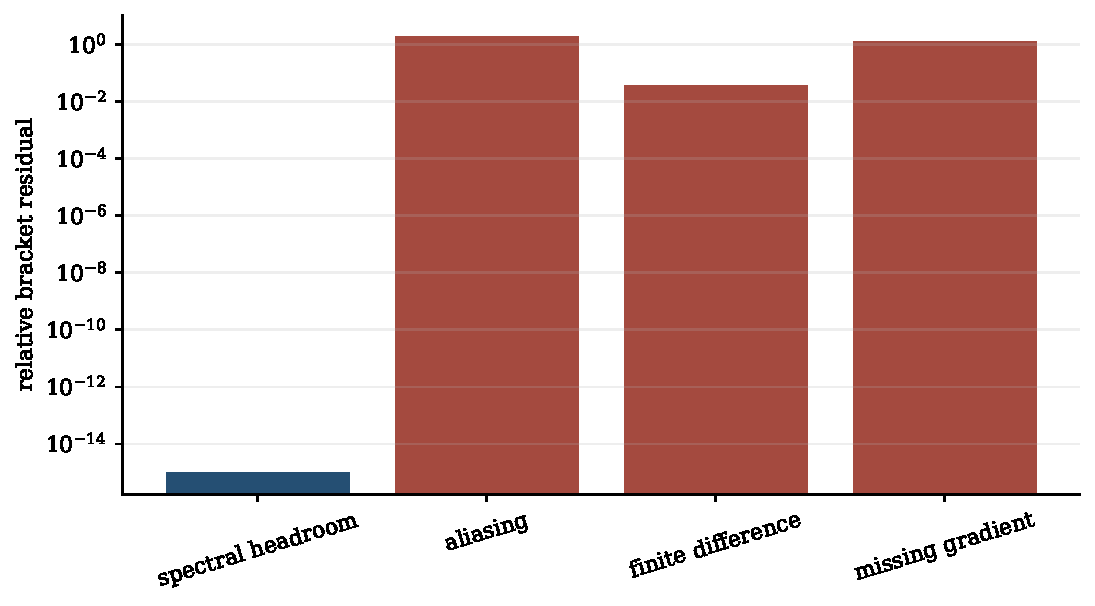
\includegraphics[width=0.93\linewidth]{constraint_negative_controls.pdf}
\caption{The scalar-fiber Hamiltonian bracket closes in the resolved spectral regime.  Aliasing, a derivative without an exact product rule, and an incomplete detail constraint all produce large defects.}
\label{fig:constraint-negative-controls}
\end{figure}

These tests are stronger than substituting one favorable trajectory.  They show that the small residual is tied to the theorem's structural assumptions.

\section{Relation to the polynomial Lorentzian parent}

The first-order matter action \eqref{eq:cov-first-order} can be appended to the existing Einstein--Cartan parent before the $3+1$ split.  The normal tetrad multiplier then receives one additional scalar-fiber constraint, while tangential diffeomorphisms receive \eqref{eq:adm-dmatter} after regular reduction.  Level rotations commute with Lorentz transformations and spacetime diffeomorphisms.

At finite spectral resolution, the complete polynomial BV master identity transfers whenever every monomial generated by the action and antibracket lies below Nyquist.  A conservative headroom rule can be obtained by counting the eight-field potential monomial together with antifield variations.  This rule is sufficient rather than sharp.  Strict finite-range locality, a quantum BV measure, and uniform continuum estimates remain separate tasks.

\section{What has and has not been closed}

\begin{longtable}{@{}P{0.45\textwidth}P{0.19\textwidth}P{0.26\textwidth}@{}}
\toprule
Statement & Status & Boundary\\
\midrule
finite-depth covariant scalar-fiber action & closed & classical EFT\\
total stress conservation & closed & on shell\\
average-detail exchange law & closed & exact at finite depth\\
matter $H$--$H$ bracket and total ADM algebra & closed & regular classical chart with gravity included\\
resolved matter Hamiltonian bracket & closed conditional & alias-free spectral headroom\\
polynomial first-order parent & closed & nondegenerate tetrad chart\\
strict finite-range nonlinear realization & open & corner-to-continuum construction required\\
quantum master equation and anomaly & open & regulator and measure required\\
self-consistent production state & open & addressed diagnostically in \Cref{ch:backreaction}\\
\bottomrule
\end{longtable}

\chapter{Arbitrary-Order Production and Fixed-Prime Sampling}
\label{ch:universality}

\section{Continuous density-of-states interpolation}

Let
\begin{equation}
\alpha:=\frac1\sigma,
\qquad
m_h\simeq\Lambda p^{\sigma h},
\qquad
N_h=p^h-1.
\label{eq:univ-alpha}
\end{equation}
Interpolating the endpoint counting function gives
\begin{equation}
N_{\mathrm c}(m)=\left(\frac m\Lambda\right)^\alpha-1,
\qquad
\frac{\dd N_{\mathrm c}}{\dd m}
=\frac1{\sigma\Lambda^\alpha}m^{\alpha-1}.
\label{eq:univ-cont-count}
\end{equation}
This defines a continuous model.  It is exact as an interpolation of the endpoint law.  \Cref{sec:univ-fixed-prime} shows why it is not an ordinary pointwise limit of a fixed-prime tower.

At a prescribed linear crossing, take
\begin{equation}
\nu(m)=Am,
\qquad
f(k,m)=\eta\exp\left[-\pi\left(\frac mA+\frac{k^2}{Am}\right)\right].
\label{eq:univ-distribution}
\end{equation}
The Gaussian momentum integral gives the number spectrum
\begin{equation}
\boxed{
\frac{\dd n}{\dd m}
=\frac{\eta A^{3/2}}
{8\pi^3\sigma\Lambda^\alpha}
m^{\alpha+1/2}\ee^{-\pi m/A}.}
\label{eq:univ-number-spectrum}
\end{equation}
Multiplication by $m$ gives the captured rest-energy spectrum
\begin{equation}
\boxed{
\frac{\dd\rho_R}{\dd m}
=\frac{\eta A^{3/2}}
{8\pi^3\sigma\Lambda^\alpha}
m^{\alpha+3/2}\ee^{-\pi m/A}.}
\label{eq:univ-rest-spectrum}
\end{equation}

\section{Exact arbitrary-order constants}

\begin{theorem}[Continuous arbitrary-order production]
For $\sigma>0$, the continuous model \eqref{eq:univ-cont-count}--\eqref{eq:univ-distribution} has
\begin{align}
n_\star
&=C_N(\sigma)\eta\frac{A^{\alpha+3}}{\Lambda^\alpha},
&C_N(\sigma)
&=\frac{\Gamma(\alpha+\tfrac32)}
{8\sigma\pi^{\alpha+9/2}},
\label{eq:univ-CN}\\
\rho_{R,\star}
&=C_R(\sigma)\eta\frac{A^{\alpha+4}}{\Lambda^\alpha},
&C_R(\sigma)
&=\frac{\Gamma(\alpha+\tfrac52)}
{8\sigma\pi^{\alpha+11/2}},
\label{eq:univ-CR}\\
\rho_\star
&=C_E(\sigma)\eta\frac{A^{\alpha+4}}{\Lambda^\alpha},
&C_E(\sigma)
&=\frac{\Gamma(\alpha+4)B(\tfrac32,\alpha+2)}
{4\sigma\pi^{\alpha+6}},
\label{eq:univ-CE}\\
p_\star
&=C_P(\sigma)\eta\frac{A^{\alpha+4}}{\Lambda^\alpha},
&C_P(\sigma)
&=\frac{C_E(\sigma)}{2\alpha+7}.
\label{eq:univ-CP}
\end{align}
Consequently,
\begin{equation}
\boxed{
w_\star(\sigma)=\frac1{7+2/\sigma},}
\label{eq:univ-w}
\end{equation}
\begin{equation}
\boxed{
f_R(\sigma)=\frac{\rho_{R,\star}}{\rho_\star}
=\frac{C_R(\sigma)}{C_E(\sigma)},}
\label{eq:univ-rest-frac}
\end{equation}
and
\begin{equation}
\boxed{
\frac{\rho_{R,\star}}{n_\star}
=m_{\mathrm{peak}}^{(R)}
=\frac A\pi\left(\frac1\sigma+\frac32\right).}
\label{eq:univ-peak}
\end{equation}
\end{theorem}

\begin{proof}
Equations \eqref{eq:univ-CN} and \eqref{eq:univ-CR} follow by integrating \eqref{eq:univ-number-spectrum} and \eqref{eq:univ-rest-spectrum} with the gamma integral.

For total energy and pressure, set $k=m\sinh\theta$.  The production exponent becomes
\begin{equation}
\pi\frac mA\cosh^2\theta.
\end{equation}
After the mass integral, the energy angular factor is
\begin{equation}
I_E=\int_0^\infty
\sinh^2\theta\cosh^{-2\alpha-6}\theta\,\dd\theta
=\frac12B\left(\frac32,\alpha+2\right).
\end{equation}
The pressure angular factor is
\begin{equation}
I_P=\frac13\int_0^\infty
\sinh^4\theta\cosh^{-2\alpha-8}\theta\,\dd\theta
=\frac16B\left(\frac52,\alpha+2\right).
\end{equation}
Their ratio is
\begin{equation}
\frac{I_P}{I_E}
=\frac13\frac{B(\tfrac52,\alpha+2)}{B(\tfrac32,\alpha+2)}
=\frac1{2\alpha+7},
\end{equation}
which proves \eqref{eq:univ-w}.  The gamma recurrence gives the mean rest mass, and differentiating \eqref{eq:univ-rest-spectrum} gives the same value for its peak.
\end{proof}

At $\sigma=1$, these formulas reduce to
\begin{equation}
w_\star=\frac19,
\qquad
f_R=\frac{525\pi}{2048},
\qquad
m_{\mathrm{peak}}^{(R)}=\frac{5A}{2\pi}.
\end{equation}

\begin{figure}[htbp]
\centering
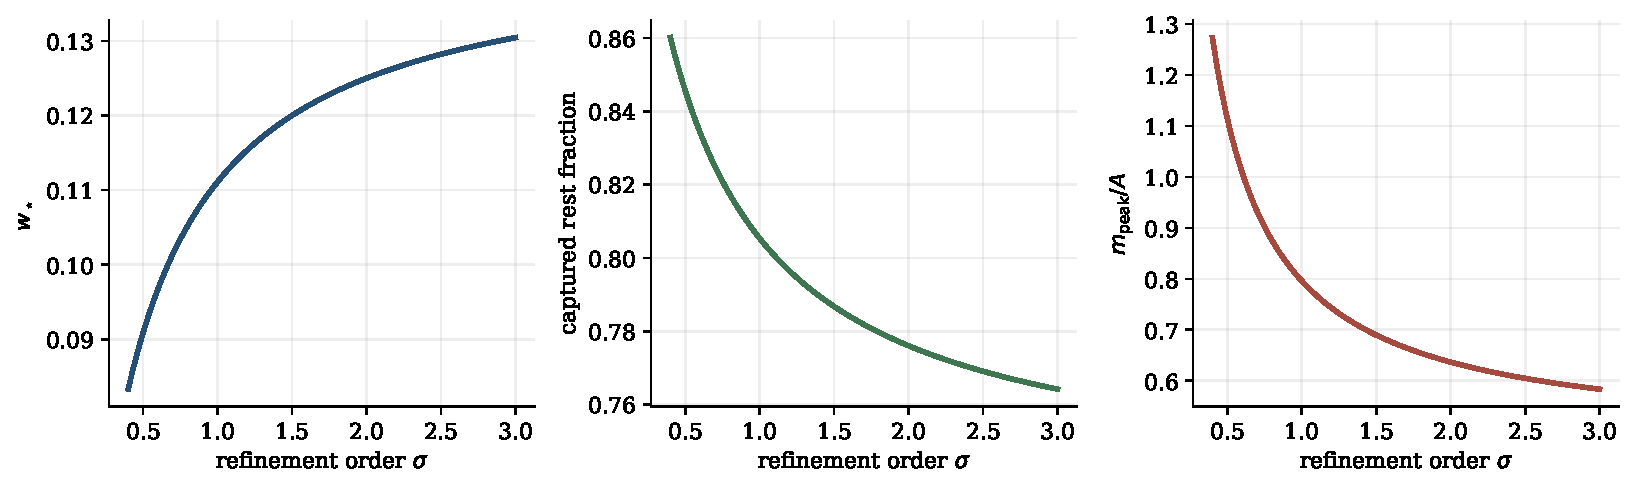
\includegraphics[width=0.98\linewidth]{general_sigma_universality.pdf}
\caption{The continuous arbitrary-order family.  Increasing $\sigma$ raises the production equation of state while lowering the captured rest fraction and the selected mass in units of $A$.}
\label{fig:general-sigma}
\end{figure}

\section{Prime independence of the interpolation}

The prime $p$ cancels from \eqref{eq:univ-cont-count} because
\begin{equation}
p^h=\left(\frac{m_h}{\Lambda}\right)^{1/\sigma}.
\end{equation}
This gives a continuous universality class labeled by $\sigma$.  Prime independence at this stage does not mean that the discrete tower forgets $p$.  The spacing in $\log m$ is $\sigma\log p$, which remains finite when $\Lambda/A$ is reduced.

\section{Fixed-prime Mellin correction}
\label{sec:univ-fixed-prime}

Let $F(y)$ be a single-state dimensionless observable with $y=m/A$, and define
\begin{equation}
x=\frac\Lambda A,
\qquad
c_p=\frac{p-1}{p},
\qquad
a=\sigma\log p.
\end{equation}
Ignoring a lower-end correction that vanishes as $x\to0$ for the production kernels, extend the level sum bilaterally:
\begin{equation}
S_F(x)=c_p\sum_{h\in\mathbb Z}p^hF(xp^{\sigma h}).
\label{eq:univ-discrete-sum}
\end{equation}
Let
\begin{equation}
\Mellin F(s)=\int_0^\infty y^{s-1}F(y)\,\dd y.
\end{equation}

\begin{theorem}[Log-periodic fixed-prime decomposition]
Suppose $F(y)=\order(y^\beta)$ as $y\to0$ for some $\beta>0$, decays sufficiently rapidly at infinity, and
\begin{equation}
g_x(t)=c_p\ee^{t\log p}F(x\ee^{at})
\end{equation}
together with its Fourier transform satisfies the integrability and summability hypotheses of Poisson summation.  A sufficient stronger condition is that $g_x$ is Schwartz.  Then
\begin{equation}
\boxed{
S_F(x)
=\frac{c_p}{a}x^{-\alpha}
\sum_{k\in\mathbb Z}
x^{\ii\omega_k}
\Mellin F(\alpha-\ii\omega_k),
\qquad
\omega_k=\frac{2\pi k}{a}.}
\label{eq:univ-mellin-poisson}
\end{equation}
\end{theorem}

\begin{proof}
Apply Poisson summation to
\begin{equation}
g(t)=c_p\ee^{t\log p}F(x\ee^{at}).
\end{equation}
In the Fourier transform, substitute $y=x\ee^{at}$.  The factor $\ee^{-2\pi\ii kt}$ becomes $(y/x)^{-\ii\omega_k}$, and the remaining integral is the Mellin transform in \eqref{eq:univ-mellin-poisson}.  The small-$y$ hypothesis also bounds the omitted physical levels $h\le0$.  Their absolute contribution is $\order(x^\beta)$ and is negligible relative to the $x^{-\alpha}$ leading abundance.
\end{proof}

The $k=0$ term has coefficient
\begin{equation}
\frac{c_p}{\sigma\log p}x^{-\alpha}\Mellin F(\alpha).
\label{eq:univ-zero-harmonic}
\end{equation}
The derivative interpolation \eqref{eq:univ-cont-count} instead has coefficient
\begin{equation}
\frac1\sigma x^{-\alpha}\Mellin F(\alpha).
\end{equation}
Their mean amplitude ratio is
\begin{equation}
\boxed{
\frac{c_p}{\log p}
=\frac{p-1}{p\log p}.}
\label{eq:univ-amplitude-ratio}
\end{equation}
It approaches one only in a formal dense-branching limit $p\to1$, not along the physical prime sequence.  The $k\ne0$ terms add a periodic dependence on $\log x$.

\begin{corollary}[No fixed-prime convergence to the derivative interpolation]
After the natural $x^\alpha$ rescaling, reducing $\Lambda/A$ at fixed $p$ translates the sampling grid in $\log m$ but does not shrink its spacing.  The rescaled discrete normalization therefore retains a prime-dependent mean offset and log-periodic corrections rather than converging to the derivative interpolation.  Ratios of observables can nevertheless be much more accurate because common amplitude factors cancel.
\end{corollary}

\clearpage
\begin{figure}[htbp]
\centering
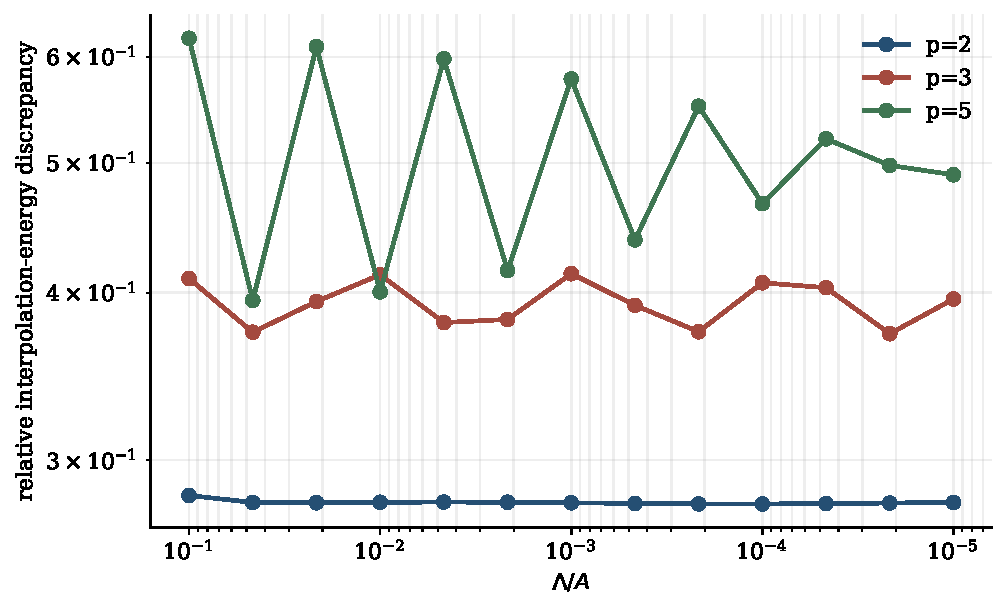
\includegraphics[width=0.82\linewidth]{fixed_prime_log_sampling.pdf}
\caption{Relative discrepancy between the discrete total production energy and the derivative interpolation at $\sigma=1$.  Decreasing $\Lambda/A$ does not remove the fixed logarithmic spacing.  The nearly constant dyadic offset and the larger prime-dependent oscillations agree with the Mellin decomposition.}
\label{fig:fixed-prime-sampling}
\end{figure}

\section{Correction to the interpretation of the continuum formulas}

The continuous constants remain exact for the density-of-states model defined by \eqref{eq:univ-cont-count}.  They also organize robust ratios in the dense mass band.  They should not be described as a convergent fixed-prime limit without an additional averaging operation, a refinement in logarithmic spacing, or a theorem that suppresses the nonzero Mellin harmonics.

This distinction matters most for absolute abundance.  The cosmological benchmark uses the direct discrete tower calculation when imposing its energy projection, so its discrete normalization is not replaced by the continuous coefficient.  The estimate explains why the reported dyadic ratios can be close to the continuous values even though the absolute energy coefficient differs substantially.

\chapter{Production Backreaction and the Frozen Benchmark}
\label{ch:backreaction}

\section{Control conditions for the rapid-crossing spectrum}

The Gaussian occupation \eqref{eq:univ-distribution} follows from a prescribed approximately linear crossing.  Three independent small parameters are required near the populated band:
\begin{equation}
\epsilon_H
:=\frac{H_\star^2}{A_\star m_{\mathrm{peak}}}\ll1,
\label{eq:back-hubble-control}
\end{equation}
\begin{equation}
\epsilon_{\mathrm{lin}}
:=\frac{|\ddot\phi_\star|}
{|\dot\phi_\star|\sqrt{A_\star m_{\mathrm{peak}}}}\ll1,
\label{eq:back-linear-control}
\end{equation}
\begin{equation}
\epsilon_{\mathrm{br}}
:=\frac{\widetilde\rho_\star}{K_\star}\ll1.
\label{eq:back-br-control}
\end{equation}
The first two control expansion and curvature across the event.  The third controls depletion by the produced modes.  A posteriori normalization cannot replace \eqref{eq:back-br-control} because depletion changes the background that generated the Bogoliubov coefficients.

\section{Benchmark energy-overdraw theorem}

The benchmark with $\lambda=1$ defines a shape-preserving projection
\begin{equation}
f_h(k)\longmapsto\eta f_h(k),
\qquad
\eta=\min\left(1,\frac{K_\star}{\widetilde\rho_\star}\right).
\label{eq:back-projection}
\end{equation}

\begin{theorem}[Failure of negligible backreaction]
For the specified benchmark record,
\begin{equation}
\eta=\BridgeEta
\end{equation}
and therefore
\begin{equation}
\boxed{
\epsilon_{\mathrm{br}}
=\frac1\eta
=\BridgeOverdraw.}
\label{eq:back-overdraw}
\end{equation}
The benchmark is outside the negligible-backreaction domain by more than twenty orders of magnitude.
\end{theorem}

\begin{proof}
The value of $\eta$ is read from the frozen discrete-tower calculation.  On the active branch of \eqref{eq:back-projection}, $\eta=K_\star/\widetilde\rho_\star$.  Inversion gives \eqref{eq:back-overdraw}.
\end{proof}

\begin{negativebox}[Physical consequence]
The exact ratios $w_\star=1/9$ and $f_R=525\pi/2048$ are properties of the projected continuous ansatz at $\sigma=1$.  They are not predictions of the coupled crossing until a backreacting solution reproduces the same spectral shape.  With $\epsilon_{\mathrm{br}}\gg1$, strong depletion is mandatory.
\end{negativebox}

\section{Hubble-loss correction before the crossing}

If the average field begins at rest at $\phi_i$ and reaches $\phi=0$, the mechanical crossing energy in FLRW obeys
\begin{equation}
\boxed{
K_{\star^-}
=U(\phi_i)-U(0)
-3\int_{t_i}^{t_\star}H\dot\phi^2\,\dd t
-E_{\mathrm{other}},}
\label{eq:back-hubble-loss}
\end{equation}
where $E_{\mathrm{other}}$ denotes the integrated work removed from the average field before the crossing.  It need not equal the final redshifted energy density of the receiving sector.  The formula without the integral is exact only in a negligible-expansion and negligible-transfer limit.  The benchmark does not fix the absolute ratio $\mu/H_\star$, so that approximation cannot be checked from the dimensionless record alone.

\section{Continuous order-one backreaction estimate}

In the arbitrary-order continuous model,
\begin{equation}
\widetilde\rho_\star
=C_E(\sigma)\frac{A^{\alpha+4}}{\Lambda^\alpha},
\qquad
K_\star=\frac{v^2A^2}{2\gamma},
\qquad \gamma>0.
\end{equation}
Introduce
\begin{equation}
a=\frac A\mu,
\qquad
\ell=\frac\Lambda\mu,
\qquad
\frac{v^2}{\mu^2}=\frac1\lambda.
\end{equation}
The raw continuous overdraw is
\begin{equation}
R_{\mathrm c}(a)
=2\gamma\lambda C_E(\sigma)
\frac{a^{\alpha+2}}{\ell^\alpha}.
\end{equation}
For the frozen dimensionless input, $R_{\mathrm c,in}=\BridgeContinuumOverdraw$.  If changing $A$ were the only response, the order-one boundary $R_{\mathrm c}=1$ would satisfy
\begin{equation}
\boxed{
\frac{A_{\mathrm{br,c}}}{A_{\mathrm{in}}}
=R_{\mathrm c,in}^{-1/(\alpha+2)}.}
\label{eq:back-cont-slow}
\end{equation}
For the benchmark, $\alpha=1$ and
\begin{align}
\frac{A_{\mathrm{br,c}}}{A_{\mathrm{in}}}
&=\BridgeContinuumSlow,\\
\frac{A_{\mathrm{br,c}}}{\mu}
&=\BridgeContinuumA,\\
\frac{\Lambda}{A_{\mathrm{br,c}}}
&=\BridgeContinuumX.
\end{align}
The lightest level would then have suppression exponent
\begin{equation}
\pi\frac{m_1}{A_{\mathrm{br,c}}}
\simeq\BridgeContinuumExponent.
\label{eq:back-cont-exponent}
\end{equation}
The continuous populated-band approximation is self-inconsistent at that point.  This is not a paradox.  It says that slowing the same continuous spectrum cannot reach its order-one boundary while holding the microscopic tower fixed.  The raw continuous coefficient is used here rather than the fixed-prime projection factor $\eta$.

\section{Direct discrete order-one threshold}

The next calculation keeps the benchmark's fixed $\Lambda$, $p$, $\sigma$, $\gamma$, $v$, and Gaussian single-crossing formula.  It changes only $A$ and evaluates the cutoff-controlled discrete momentum moments.  Define
\begin{equation}
R_{\mathrm{disc}}(A)
:=\frac{\widetilde\rho_{\mathrm{disc}}(A)}{v^2A^2/(2\gamma)}.
\label{eq:back-Rdisc}
\end{equation}

\begin{diagnostic}[Discrete backreaction threshold]
The equation $R_{\mathrm{disc}}(A)=1$ has the numerical solution
\begin{equation}
\boxed{
\frac{A_{\mathrm{br,d}}}{\mu}=\BridgeDiscreteA,
\qquad
\frac{\Lambda}{A_{\mathrm{br,d}}}=\BridgeDiscreteX.}
\label{eq:back-disc-sat}
\end{equation}
At this point,
\begin{equation}
\boxed{
w_{\mathrm{br,d}}=\BridgeDiscreteW,
\qquad
f_{R,\mathrm{br,d}}=\BridgeDiscreteRest,
\qquad
\frac{\langle m\rangle_R}{A}=\BridgeDiscreteMeanMass.}
\label{eq:back-disc-ratios}
\end{equation}
\end{diagnostic}

The calculation uses 128-node generalized Gauss--Laguerre momentum quadrature and the exact discrete degeneracies.  Three levels fall below the declared suppression cutoff.  The first carries essentially all of the production weight.

\begin{figure}[htbp]
\centering
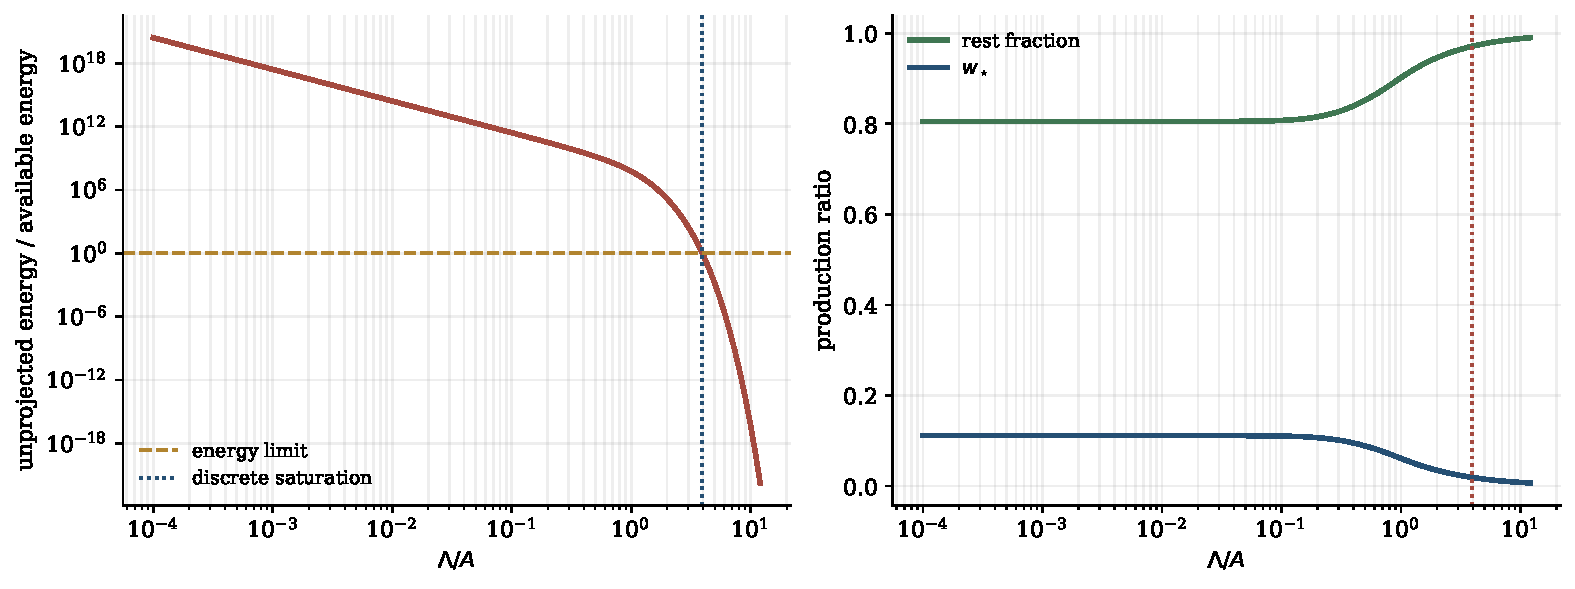
\includegraphics[width=0.98\linewidth]{backreaction_obstruction.pdf}
\caption{Left: the unprojected energy relative to the crossing reservoir as $\Lambda/A$ is increased at fixed microscopic $\Lambda$.  The order-one backreaction threshold occurs after the continuous populated-band regime has been left.  Right: the production state becomes more rest dominated and its pressure falls as the tower sparsifies.}
\label{fig:backreaction-obstruction}
\end{figure}

\begin{statusbox}[Diagnostic boundary]
Equation \eqref{eq:back-disc-sat} is not a time-dependent backreaction solution and is not an energy-partition equation for the original crossing.  It marks where the prescribed spectrum and kinetic reservoir become comparable inside a one-parameter Gaussian family.  Its value is useful because the family has already become sparse and cold at that boundary.  A dynamical solution can depart further.
\end{statusbox}

\section{Interaction-strength obstruction}

For a detail eigenvalue $\lambda_h=\Lambda^2p^{2\sigma h}$, the canonical four-dimensional action contains the quartic interaction
\begin{equation}
-\frac12g_h\phi^2\chi_h^2,
\qquad
g_h=\gamma\frac{\lambda_h}{v^2}.
\label{eq:back-gh}
\end{equation}
Using $v^2=\mu^2/\lambda$ and $m_h^2\simeq\lambda_h$ gives
\begin{equation}
g_h\simeq\gamma\lambda\left(\frac{m_h}{\mu}\right)^2.
\label{eq:back-gh-scaled}
\end{equation}
At the frozen discrete peak with $\gamma=16$ and $\lambda=1$,
\begin{equation}
\boxed{g_{\mathrm{peak}}\simeq\BridgePeakCoupling.}
\label{eq:back-peak-coupling}
\end{equation}
A nominal loop-control condition $g_{\mathrm{peak}}<1$ would instead require
\begin{equation}
\lambda<\BridgeLambdaBound
\label{eq:back-lambda-bound}
\end{equation}
with the other benchmark ratios held fixed.  At $\lambda=1$, even the lightest level at the discrete threshold has
\begin{equation}
g_1\simeq\BridgeLowestCoupling.
\end{equation}

At fixed calibrated ratios $A/\mu$ and $\Lambda/\mu$, the two diagnostics are parametrically linked:
\begin{equation}
R_{\mathrm{br}}(\lambda)
=\frac{\lambda}{\lambda_{\mathrm{frozen}}}
R_{\mathrm{br}}(\lambda_{\mathrm{frozen}}).
\end{equation}
For $\lambda_{\mathrm{frozen}}=1$, avoiding energy overdraw requires
\begin{equation}
\boxed{\lambda\le\BridgeEnergyLambdaBound.}
\end{equation}
At that boundary, the peak and lightest-level couplings would be
\begin{equation}
g_{\mathrm{peak}}=\BridgePeakAtEnergyBound,
\qquad
g_1=\BridgeLowestAtEnergyBound.
\end{equation}

\begin{negativebox}[Perturbative boundary]
The printed $\lambda=1$ benchmark is neither weakly backreacting nor under loop control.  Large $g_h$ does not by itself invalidate the exact solution of a quadratic mode equation on a prescribed background.  The fixed-background approximation fails independently because of the energy overdraw.  Reducing the free quartic can cure both tree-level diagnostics along this parameter slice, but it changes the absolute scale $\mu\propto\lambda^{1/4}$ at fixed vacuum density and requires new Hubble, production, and loop checks.
\end{negativebox}

\section{Self-consistent semiclassical system}

A minimal next calculation must solve the background, modes, and geometry together.  At finite depth, one suitable Hartree system is
\begin{align}
\ddot\phi+3H\dot\phi+U'(\phi)
+\frac12F'(\phi)Y_H^{\mathrm{ren}}&=0,
\label{eq:back-hartree-phi}\\
\ddot u_{h,k}+3H\dot u_{h,k}
+\left(\frac{k^2}{a^2}+m_b^2+F(\phi)\lambda_h\right)u_{h,k}&=0,
\label{eq:back-hartree-mode}\\
3M_{\mathrm{Pl}}^2H^2
&=\frac12\dot\phi^2+U(\phi)+\rho_H^{\mathrm{ren}}+\rho_{\mathrm{vis}},
\label{eq:back-hartree-friedmann}
\end{align}
where
\begin{equation}
Y_H^{\mathrm{ren}}
=\sum_{h=1}^{H}d_h\lambda_h
\int\frac{\dd^3k}{(2\pi)^3}
\left(|u_{h,k}|^2-\text{adiabatic subtraction}\right).
\label{eq:back-Yren}
\end{equation}
The same subtraction prescription must be used in $\rho_H^{\mathrm{ren}}$.  Equations \eqref{eq:cov-cont-chi}--\eqref{eq:cov-cont-phi} then provide an exact numerical conservation test.

The calculation is not complete until it demonstrates all of the following.
\begin{enumerate}[leftmargin=2.2em]
\item cutoff stability over a declared range of $H$ and momentum resolution
\item conservation after renormalization
\item independence from an arbitrary scale-factor normalization
\item a spectral output rather than a shape-preserving projection
\item a regime in which quantum and higher-order corrections are controlled
\end{enumerate}

No result in this chapter claims that such a solution exists for the frozen parameters.  The energy and interaction-strength diagnostics make survival of that exact benchmark unlikely without a substantial microscopic revision.

\chapter{Finite-Depth Quantum Stability and Ultraviolet Growth}
\label{ch:radiative}

\section{Why finite depth is not optional}

The classical fiber operator is well defined on suitable infinite-depth domains.  A quantum effective potential asks a different question.  Every level contributes vacuum fluctuations, and the multiplicity grows with depth.  Normal ordering a produced-particle density does not remove the vacuum terms in the effective action.

The honest starting point is therefore finite $H$ with a declared physical or effective cutoff.  Let
\begin{equation}
M_h^2(\phi)=m_b^2+F(\phi)\lambda_h,
\qquad
\lambda_h=\Lambda^2p^{2\sigma h}.
\label{eq:rad-level-mass}
\end{equation}

\section{One-loop effective potential}

For canonical real bosonic detail fields on a constant background with $M_h^2(\phi)>0$, the flat-space, local-potential contribution in a standard subtraction scheme is
\begin{equation}
\boxed{
\Delta U_H(\phi)
=\frac1{64\pi^2}
\sum_{h=1}^{H}d_hM_h^4(\phi)
\left[
\log\frac{M_h^2(\phi)}{\bar\mu^2}-\frac32
\right].}
\label{eq:rad-CW}
\end{equation}
At the locked origin, $F'(0)=0$ and $F''(0)=2\gamma/v^2$.  The induced average curvature is
\begin{equation}
\boxed{
\Delta m_\phi^2
=\frac\gamma{16\pi^2v^2}
\sum_{h=1}^{H}d_h\lambda_hM_{h0}^2
\left[
\log\frac{M_{h0}^2}{\bar\mu^2}-1
\right],}
\label{eq:rad-mass-correction}
\end{equation}
where $M_{h0}^2=m_b^2+\lambda_h$.

Equation \eqref{eq:rad-mass-correction} does not by itself prove that locking fails.  Counterterms can be chosen at finite depth.  It proves that the locking curvature is radiatively sensitive to the tower unless a symmetry or ultraviolet completion controls the sum.  On a curved background, additional $M_h^2R$ and curvature-squared counterterms are required.  If a level mass becomes negative, the logarithm develops an imaginary part and the expression is not a real stability potential.

\section{Infinite-depth growth theorem}

\begin{theorem}[Bosonic tower ultraviolet growth]
Fix $\phi$ with $F(\phi)>0$.  For $\sigma>0$ and large depth,
\begin{equation}
\sum_{h=1}^{H}d_hM_h^4
\asymp
F(\phi)^2\Lambda^4p^{(1+4\sigma)H}.
\label{eq:rad-geometric-growth}
\end{equation}
Writing
\begin{equation}
M_{\mathrm{UV}}=\Lambda p^{\sigma H},
\end{equation}
the leading power is
\begin{equation}
\boxed{
\Delta U_H
\sim
\frac{M_{\mathrm{UV}}^{4+1/\sigma}}
{\Lambda^{1/\sigma}}}
\label{eq:rad-UV-power}
\end{equation}
up to logarithms and scheme-dependent coefficients.
\end{theorem}

\begin{proof}
At high level, $d_h\sim p^h$ and $M_h^4\sim F(\phi)^2\Lambda^4p^{4\sigma h}$.  Their product is a geometric sequence with ratio $p^{1+4\sigma}$.  The last term controls the finite sum.  Substituting $p^H=(M_{\mathrm{UV}}/\Lambda)^{1/\sigma}$ gives \eqref{eq:rad-UV-power}, with the fixed factor $F(\phi)^2$ suppressed there.  If $F=0$, the base mass instead gives growth proportional to $p^H$.  If $F<0$, sufficiently high levels are tachyonic.
\end{proof}

\begin{figure}[htbp]
\centering
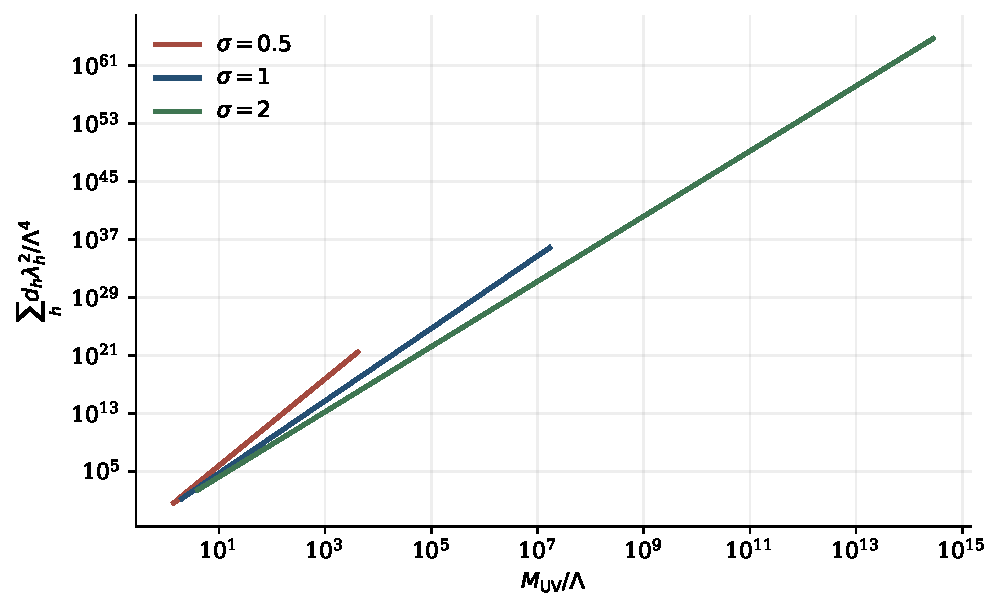
\includegraphics[width=0.82\linewidth]{radiative_uv_growth.pdf}
\caption{The multiplicity-weighted fourth mass moment at finite depth.  The fitted slopes agree with $4+1/\sigma$.  The lines have different horizontal ranges because the same depth produces different ultraviolet masses.}
\label{fig:radiative-growth}
\end{figure}

\begin{negativebox}[Ultraviolet boundary]
The ordinary bosonic infinite tower does not have a finite one-loop potential without a physical cutoff, cancellations, or a different spectral ultraviolet prescription.  Classical Hilbert-space convergence does not supply that cancellation.
\end{negativebox}

\section{Radiative closure of the one-coupling pattern}

At tree level, the level interaction coefficients obey
\begin{equation}
g_h=\gamma\frac{\lambda_h}{v^2}.
\end{equation}
A generic finite multiscalar quantum theory produces counterterms of the forms
\begin{equation}
\phi^4,
\qquad
\chi_h^4,
\qquad
\chi_h^2\chi_j^2,
\qquad
\phi^2\chi_h^2,
\end{equation}
with independent finite parts unless a symmetry relates them.  Level-orthogonal invariance constrains indices within one level.  Branch homogeneity relates levels only if the regulator and renormalization prescription preserve the branching maps.  A finite upper boundary introduces additional endpoint terms.

The single $\gamma$ statement applies only to the order-$2\sigma$ spectral channel of the classical ansatz.  The allowed order-zero coefficient $\kappa$ was set to zero as a model restriction, and generic loop corrections need not preserve that restriction.  There is no renormalization theorem yet.  A completed model needs one of the following:
\begin{enumerate}[leftmargin=2.2em]
\item a physical finite-depth endpoint
\item paired degrees of freedom that cancel the leading vacuum moments
\item an ultraviolet fixed point with a proved invariant counterterm family
\item a modulus or gauge principle that turns the coefficient pattern into a protected geometric quantity
\end{enumerate}

\section{A dynamical refinement-scale modulus}

One candidate completion promotes the multiplier of $L_H$ to a field.  Introduce a canonical scalar $s$ and define
\begin{equation}
\begin{aligned}
S_H^{\mathrm{mod}}=\int\sqrt{-g}\,\dd^4x\Bigg[
&\frac{M_{\mathrm{Pl}}^2}{2}R
-\frac12(\nabla\phi)^2-U(\phi)
-\frac12(\nabla s)^2-W(s,\phi)\\
&-\frac12\ip{\nabla\chi}{\nabla\chi}_H
-\frac12\ip{\chi}{\left(m_b^2+\ee^{2s/f_s}L_H\right)\chi}_H
\Bigg].
\end{aligned}
\label{eq:rad-modulus-action}
\end{equation}
Choose
\begin{equation}
W(s,\phi)
=\frac{M_s^2}{2}
\left[
s-\frac{f_s}{2}\log F(\phi)
\right]^2.
\label{eq:rad-modulus-potential}
\end{equation}

\begin{proposition}[Heavy-modulus matching]
If
\begin{equation}
M_s^2\gg H^2,
\qquad
M_s^2\gg A_\star m_{\mathrm{peak}},
\qquad F>0,
\qquad
|\Box s_0|\ll f_sM_s^2,
\qquad
F Y_H\ll f_s^2M_s^2,
\label{eq:rad-heavy-conditions}
\end{equation}
where $s_0(\phi)=\tfrac{f_s}{2}\log F(\phi)$.  Then the modulus equation has the adiabatic solution
\begin{equation}
s=s_0
+\frac{\Box s_0}{M_s^2}
-\frac{FY_H}{f_sM_s^2}
+\order(M_s^{-4}),
\label{eq:rad-s-solution}
\end{equation}
and hence
\begin{equation}
\ee^{2s/f_s}
=F(\phi)
\left[
1+\order\left(\frac{\Box s_0}{f_sM_s^2},
\frac{FY_H}{f_s^2M_s^2}\right)
\right].
\label{eq:rad-modulus-match}
\end{equation}
\end{proposition}

\begin{proof}
Expand the modulus equation around the moving minimum of \eqref{eq:rad-modulus-potential}.  To leading order it is $\Box s_0-M_s^2(s-s_0)-FY_H/f_s=0$, which gives \eqref{eq:rad-s-solution}.  Expanding the exponential gives \eqref{eq:rad-modulus-match}.
\end{proof}

\begin{statusbox}[Model status]
The proposition matches the detail mass multiplier, not the complete original scalar EFT.  Substituting the moving minimum also produces the unsuppressed operator
\begin{equation}
-\frac12(\nabla s_0)^2
=-\frac{f_s^2}{8}(\nabla\log F)^2.
\end{equation}
It must be retained or shown negligible.  The chosen potential \eqref{eq:rad-modulus-potential} remains a model input.  It does not derive $\gamma$, and it does not cancel the tower vacuum energy by itself.
\end{statusbox}

\section{Quantum tasks that remain}

The next quantum block must supply a regulator compatible with diffeomorphism and internal symmetries, a finite counterterm basis, a measure contribution in the BV pushforward, and a cutoff-stable prediction.  It must also decide whether $H$ is physical, emergent, or removed through a cancellation.  Until then, infinite-depth statements should be restricted to the classical operator domains for which they were proved.

\chapter{Physical Interpretation and Unresolved Comparisons}
\label{ch:assessment}

\section{Mathematical construction and physical validation}

A coherent mathematical construction, a controlled physical model, and an empirically supported theory are different kinds of result. The finite-depth covariant and canonical identities concern a stated model. The production spectrum additionally requires a controlled solution of the coupled dynamics. Empirical identification requires comparison with data and competing models.

The energy-budget obstruction locates a failure in the specified production history. It does not invalidate projector reconstruction, matrix-corner calculus, or the conditional transport of a prescribed distribution. It does prevent that distribution from being called a prediction of the microscopic crossing without a new dynamical argument.

\section{Established model statements}

The central results separate symmetry, conservation, approximation, and physical production.

\begin{longtable}{@{}P{0.36\textwidth}P{0.20\textwidth}P{0.34\textwidth}@{}}
\toprule
Result & Status & Scientific role\\
\midrule
Level-orthogonal quadratic operator classification & theorem & isolates one coefficient per refinement level\\
Branch-homogeneity recurrence & theorem & reduces those coefficients to one geometric family\\
Leading analytic spectral interaction & theorem within stated parity, locality, and exact-order assumptions & explains one channel but leaves an allowed order-zero coupling\\
Covariant stress-exchange identity & theorem & supplies an exact conservation diagnostic\\
Total hypersurface algebra with scalar fiber & theorem & shows that the finite-depth matter sector is canonically compatible after gravity is included\\
Resolved matter $H$--$H$ test and negative controls & controlled diagnostic & separates spectral headroom from aliasing and omitted-gradient failures\\
Arbitrary-order continuum moments & theorem for the interpolated density model & extends the production ratios beyond \(\sigma=1\)\\
Fixed-prime Mellin decomposition & theorem & corrects the interpretation of the continuum approximation\\
Specified benchmark energy audit & controlled diagnostic & proves the prescribed crossing is not weakly backreacting\\
Finite-depth one-loop power counting & theorem at leading ultraviolet order & exposes the need for a cutoff or cancellation\\
Heavy-modulus realization & model proposition & supplies a testable route to a common scale multiplier\\
\bottomrule
\end{longtable}

The energy-budget result is a central obstruction.  The specified rapid-crossing spectrum is not a small perturbation of its background.  Its unprojected energy exceeds the declared reservoir by \(\BridgeOverdraw\).  A free crossing followed by a common normalization factor therefore cannot be read as a self-consistent production history.

This negative result is constructive.  It localizes the failure upstream of the late transport calculation and gives exact equations for replacing the projection.  It also prevents further phenomenology from accumulating on an uncontrolled microscopic input.

\section{Limits of the model}

The following claims remain outside the proved domain.
\begin{enumerate}[leftmargin=2.2em]
\item The projector axioms do not select \(p\), \(\sigma\), \(\Lambda\), \(m_b\), \(\gamma\), the potential parameters, or the initial state.
\item The symmetry classification does not calculate the numerical value \(\gamma=16\).
\item The order-one backreaction threshold is not a solution of the coupled background and mode equations or an energy-partition equation.
\item The projected Gaussian ratios are not preserved under strong backreaction unless a dynamical calculation demonstrates that fact.
\item The ordinary infinite bosonic tower is not radiatively finite under the finite-depth continuation studied here.
\item The modulus completion does not solve the cosmological constant problem or prove ultraviolet completeness.
\item The internal verification archive is not independent reproduction, peer review, or experimental evidence.
\item No dark matter or dark energy identification follows solely from a match to a prescribed background abundance.
\end{enumerate}

\section{A controlled production comparison}

An additional observable template does not resolve the upstream production problem.  It is a finite-depth backreacting production calculation with one conserved renormalized stress tensor.  The system in \eqref{eq:back-hartree-phi}--\eqref{eq:back-hartree-friedmann} is the minimum viable model.

The calculation should be organized as a sequence of gates.

\begin{longtable}{@{}P{0.13\textwidth}P{0.35\textwidth}P{0.42\textwidth}@{}}
\toprule
Gate & Required result & Failure meaning\\
\midrule
G1 & Renormalized total continuity residual converges to zero with time step and momentum resolution & implementation or subtraction is inconsistent\\
G2 & Observables stabilize across at least three finite depths and two momentum cutoffs & prediction is regulator dominated\\
G3 & The produced spectrum is obtained from the coupled evolution without a common post hoc projection & microscopic production is actually solved\\
G4 & Interaction and loop expansion parameters are below declared bounds, or a nonperturbative method is used & free-mode interpretation is invalid\\
G5 & A viable region reproduces abundance, pressure, and coldness simultaneously & the proposed cosmological branch survives\\
G6 & At least one linked observable differs from a simpler model after nuisance parameters are fit & the construction becomes falsifiable rather than only flexible\\
\bottomrule
\end{longtable}

\begin{negativebox}[Go or revise]
If no cutoff-stable solution passes G1--G5, the specified cosmological branch should be revised or retired.  The projector, corner, and constrained-system results would remain as separate mathematical work.  A failed dark-sector realization would not invalidate them.
\end{negativebox}

\section{Minimum computational experiment}

A credible first run does not need the full infinite tower.  It needs a converged finite-depth sequence.

\begin{enumerate}[leftmargin=2.2em]
\item Choose \(H=1,2,3,4\) and publish the physical largest mass at every depth.
\item Initialize fourth-order adiabatic vacuum modes over a documented comoving momentum grid.
\item Use the same adiabatic subtraction terms in \(Y_H^{\mathrm{ren}}\), \(\rho_H^{\mathrm{ren}}\), and \(p_H^{\mathrm{ren}}\).
\item Evolve \(\phi\), all retained modes, and the Friedmann equation together through the crossing.
\item Monitor the covariant identity in \eqref{eq:cov-ward} and the FLRW exchanges in \eqref{eq:cov-exchange-chi}--\eqref{eq:cov-exchange-phi} at every step.
\item Repeat with doubled time resolution, doubled momentum resolution, and shifted ultraviolet cutoffs.
\item Report the unprojected spectrum, energy, pressure, rest fraction, level occupancy, and their convergence envelopes.
\item Scan \(\lambda\), \(\gamma\), \(\Lambda/\mu\), \(m_b/\mu\), and the invariant crossing condition.  Do not use a coordinate value of the scale factor as the only clock.
\end{enumerate}

The first scientific deliverable from this experiment should be a survival map, not a best-fit point.  Its axes should distinguish the weakly coupled, strongly backreacting, tachyonic, cutoff-sensitive, and radiatively unstable regions.

\section{A second foundational track}

The strongest purely gravitational continuation is different.  It is an end-to-end nonlinear Gowdy corner--BFV continuum bridge.  That track should derive the ungauge-fixed \(T^2\)-symmetric sector from the real polynomial Lorentzian parent, construct an explicit corner derivative and variable-shift generator, instantiate a cyclic contraction, prove finite BFV nilpotency and refinement-path equivalence, and establish uniform local-in-time convergence after areal gauge on \([t_0,T]\) with \(t_0>0\).

That theorem would close the gap between the abstract matrix-corner calculus and the filtered Fourier realizations used in the later gravitational chapters.  It is the right foundational milestone alongside the matter comparison.  It should not be replaced by an unrestricted \(3+1\) or quantum claim before the symmetry-reduced continuum map is explicit.

\section{Decision table for the program}

\begin{longtable}{@{}P{0.27\textwidth}P{0.31\textwidth}P{0.32\textwidth}@{}}
\toprule
Outcome & Interpretation & Next action\\
\midrule
Backreacting spectrum remains close to the prescribed ansatz in a controlled region & cosmological bridge gains microscopic support & rerun late observables with propagated theory uncertainty\\
Spectrum survives but is substantially reshaped & mechanism may survive, benchmark does not & replace frozen initial distribution and refit every downstream stage\\
Only strongly coupled solutions exist & free production calculation is the wrong tool & formulate and validate a nonperturbative treatment\\
Finite-depth results fail to stabilize & tower prediction is regulator dependent & identify a physical endpoint or ultraviolet cancellation\\
No viable production region exists & dark-sector realization is falsified in this form & retain mathematical framework and revise the matter completion\\
Gowdy bridge succeeds independently & foundational architecture gains a nonlinear continuum theorem & extend cautiously to additional symmetry classes\\
\bottomrule
\end{longtable}

\section{Final claim boundary}

The construction supplies exact internal identities, conditional gravitational statements, and an explicitly testable fiber model. Its specified cosmological production benchmark fails a quantified energy-budget test. A viable physical realization must control backreaction, ultraviolet sensitivity, and the transport of any resulting uncertainty through the observable calculations.

The cosmology chapter therefore begins from a prescribed normalized distribution. Its deductions retain their conditional meaning. They do not assume that the unresolved production comparison has succeeded.

\appendix
\chapter{Computational Evidence and Reproducibility}
\label{app:reproducibility}

\section{Source integrity and executable provenance}

The release audit found two different kinds of evidence.  First, the Volume II source manifest is internally intact.  All $\BridgeManifestEntries$ listed entries match their recorded SHA-256 digests.  Second, the computational package does not rebuild in place without staging and inherited files.

\begin{longtable}{@{}P{0.43\textwidth}P{0.16\textwidth}P{0.31\textwidth}@{}}
\toprule
Record & Count & Meaning\\
\midrule
Volume II manifest entries verified & $\BridgeManifestEntries$ & byte integrity\\
Frozen internal checks recorded as passing & $\BridgeFrozenPasses$ & archived implementation evidence\\
Byte-identical inherited data artifacts & $\BridgeLineageData$ & cross-volume provenance\\
Byte-identical inherited figures & $\BridgeLineageFigures$ & cross-volume provenance\\
Nested scripts requiring a staging layout & $\BridgeStagingScripts$ & not runnable in place\\
Required but absent declared paths & $\BridgeMissingPaths$ & three chapter records and one release manifest\\
\bottomrule
\end{longtable}

The $\BridgeFrozenPasses$ passing checks were counted from ten archived verification summaries.  They are frozen records.  They were not all rerun from the Volume II package because the namespaced programs resolve their working root to the verification directory and then expect absent sibling data or parent inputs.  Three records named by the scale-covariant chapter are absent from that package.  Their ancestors exist in the first-volume source.  The release documents also require a release manifest that is not present.

The Volume I technical supplement contains a visible status-key typo caused by a tab escape replacing the backslash in several \texttt{\string\textbf} commands.  This bridge records the defect in an errata ledger.  The frozen release is not silently overwritten.

\begin{statusbox}[Provenance boundary]
Hash agreement proves that a file has not changed relative to its manifest.  Byte-identical inheritance proves lineage.  Neither proves that the physical assumptions are correct.  A frozen pass count is not an independent rerun.
\end{statusbox}


\section{Scope of the executable record}

The accompanying package reproduces the numerical statements associated with this model.  It also performs a read-only integrity and lineage audit of the extracted parent sources.  It does not claim to rerun every frozen parent computation.

The bridge verification has three classes of output:
\begin{enumerate}[leftmargin=2.2em]
\item analytic constants evaluated in double precision
\item resolved numerical identities and deliberately failing negative controls
\item deterministic audits of hashes, paths, and cross-volume byte lineage
\end{enumerate}

The machine-readable claim registry gives every central statement a status and a validation route.  The parameter registry separates structural choices, benchmark values, and derived quantities.

\section{Clean-run commands}

From the package root on a Unix-like system, create an isolated environment and run
\begin{verbatim}
python -m venv .venv
. .venv/bin/activate
python -m pip install -r requirements.txt
python code/verify_covariant_backreaction.py \
  --parent-json parent/Scale_Covariant_Dark_Sector_Verification.json \
  --output data --figures figures
python code/generate_latex_values.py \
  --data data --output generated_values.tex
python code/validate_release.py --root .
latexmk -pdf -interaction=nonstopmode -halt-on-error \
  -outdir=build \
  Projector_Refinement_Physics_Covariant_Backreaction_Bridge.tex
\end{verbatim}

The parent JSON is included in the source package under \texttt{parent/}.  The separate provenance audit requires extracted Volume I, Volume II, and Volume I technical-supplement source roots.  Its command and expected directory arguments are documented in \texttt{REPRODUCIBILITY.md}.

On Windows PowerShell, \texttt{build.ps1} performs the bridge verification, macro generation, validation, and PDF build after the Python environment is installed.

\section{Verification checks}

The new suite records nineteen passing checks.  Five of them are negative controls that pass only when the deliberately damaged or uncontrolled case is detected.

\begin{longtable}{@{}P{0.13\textwidth}P{0.38\textwidth}P{0.15\textwidth}P{0.24\textwidth}@{}}
\toprule
ID & Test & Result & Boundary\\
\midrule
COV01 & finite-level commutant dimension & pass & numerical linear algebra illustration\\
COV02 & refinement coefficient nullity & pass & numerical recurrence illustration\\
COV03 & FLRW exchange identity & pass & double-precision residual\\
COV04 & omitted exchange source & pass & nonzero negative control\\
ADM01 & alias-free scalar-fiber bracket & pass & residual \(\BridgeSpectralResidual\)\\
ADM02 & violated spectral headroom & pass & residual \(\BridgeAliasResidual\)\\
ADM03 & centered-difference derivative & pass & residual \(\BridgeFiniteDifferenceResidual\)\\
ADM04 & omitted detail gradient & pass & residual \(\BridgeMissingGradientResidual\)\\
UNI01 & \(\sigma=1\) closed forms & pass & four analytic constants\\
UNI02 & outer quadrature at \(\sigma=0.5\) & pass & independent continuum moments\\
UNI03 & outer quadrature at \(\sigma=1\) & pass & independent continuum moments\\
UNI04 & outer quadrature at \(\sigma=2\) & pass & independent continuum moments\\
QUA01 & 96-node versus 128-node rule & pass & energy and pressure convergence\\
BKR01 & specified benchmark energy overdraw & pass & uncontrolled production is detected\\
BKR02 & parent overdraw reconstruction & pass & direct discrete moment check\\
BKR03 & order-one threshold root & pass & \(R_{\mathrm{disc}}=1\) residual\\
BKR04 & raw-continuum identity & pass & independent continuum coefficient\\
CPL01 & nominal loop-coupling bound & pass & \(g_{\mathrm{peak}}=1\) boundary\\
CPL02 & energy-control coupling relation & pass & linked \(\lambda\) scaling\\
\bottomrule
\end{longtable}

``Pass'' for a negative control means that the deliberately damaged model produced a residual above its declared lower bound.  It does not mean that the damaged model is acceptable.

\begin{figure}[htbp]
\centering
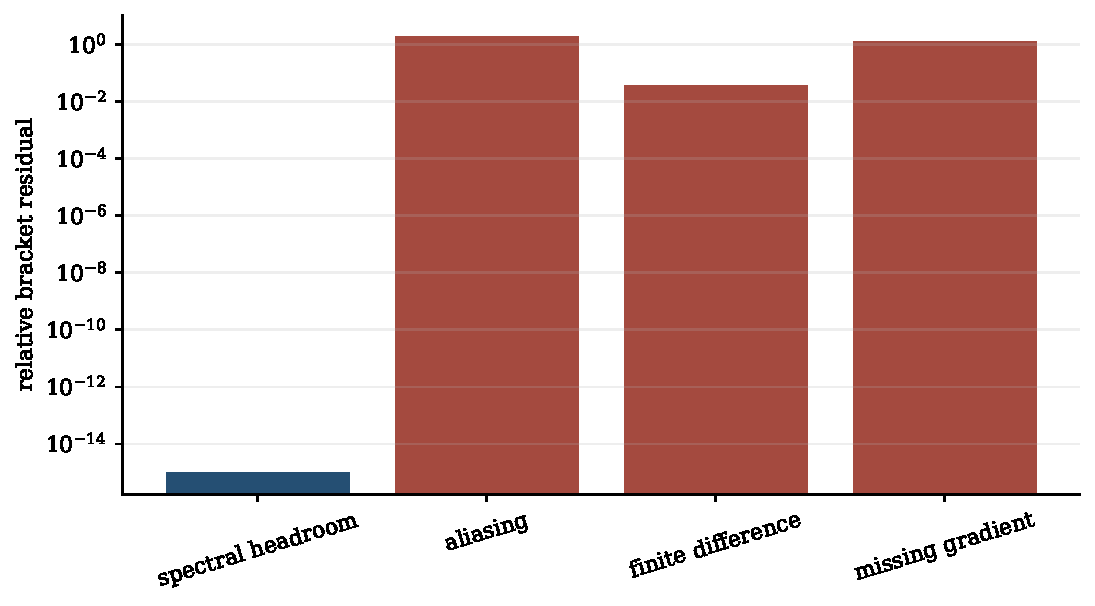
\includegraphics[width=0.84\linewidth]{constraint_negative_controls.pdf}
\caption{Resolved bracket closure and negative controls.  The alias-free spectral calculation closes near machine precision.  Aliasing, a derivative without an exact product rule on the represented algebra, and removal of the detail gradient expose distinct failures.}
\label{fig:repro-negative-controls}
\end{figure}

\section{Data products}

\begin{longtable}{@{}P{0.38\textwidth}P{0.52\textwidth}@{}}
\toprule
Path & Contents\\
\midrule
\texttt{data/verification\_checks.csv} & individual check status, residual, tolerance, and role\\
\texttt{data/verification\_summary.json} & aggregate pass count and central claim boundary\\
\texttt{data/backreaction\_audit.json} & benchmark overdraw, order-one threshold diagnostics, and coupling bounds\\
\texttt{data/continuum\_universality.csv} & arbitrary-\(\sigma\) analytic constants\\
\texttt{data/discrete\_convergence.csv} & fixed-prime discrete and interpolation comparisons\\
\texttt{data/energy\_saturation\_curve.csv} & cutoff-controlled discrete energy, pressure, and rest moments along the diagnostic scan\\
\texttt{data/radiative\_scaling.csv} & finite-depth ultraviolet moments and fitted scaling inputs\\
\path{data/frozen_verification_ledger.csv} & pass counts read from archived parent summaries\\
\texttt{data/cross\_volume\_lineage.csv} & byte-identical parent artifact pairs\\
\texttt{data/python\_staging\_audit.csv} & static root-resolution audit for namespaced programs\\
\path{data/errata_and_broken_references.csv} & missing declared paths and released erratum\\
\bottomrule
\end{longtable}

All CSV files use a header row and UTF-8 encoding.  JSON files are indented and key sorted.  Figures are emitted as both PDF and PNG from the same Python calculation.

\section{Source-archive audit}

The parent audit verifies \(\BridgeManifestEntries\) Volume II manifest entries.  It finds no digest mismatch.  It counts \(\BridgeFrozenPasses\) passing and zero failing checks across ten archived summary files.  These are frozen results, not fresh executions.

The audit also detects \(\BridgeLineageData\) data files and \(\BridgeLineageFigures\) figures in Volume II that are byte-identical to Volume I ancestors.  The result is positive provenance evidence.  It is not independent confirmation because identical bytes carry the same assumptions and implementation history.

Twelve nested Python programs require a staged directory layout to resolve their declared root.  Four declared release or chapter paths are absent.  Those conditions are retained in the ledger rather than repaired invisibly.

\section{Source erratum}
The supporting technical supplement contains malformed status-label typography. The original file is retained unchanged in the provenance archive. The defect concerns presentation rather than a mathematical identity. Source identity and the corrected reading text are recorded separately.

\clearpage
\section{Numerical methods and tolerances}

Momentum moments use a 128-node generalized Gauss--Laguerre rule with weight exponent $1/2$ after the production exponential is separated analytically.  The pressure integrand supplies one additional factor of the quadrature variable.  The discrete tower is truncated only after the dimensionless mass reaches a declared suppression cutoff.  The order-one backreaction threshold is solved by a bracketed scalar root finder.  Spectral derivatives use the periodic discrete Fourier transform.

Positive checks use tolerances appropriate to double-precision arithmetic or to the declared quadrature.  Negative controls use lower bounds rather than upper tolerances.  Every row states which direction is expected.  The package validator rejects any failed row, a disagreement between the CSV and JSON counts, or a missing central output.

The computations are deterministic.  The only randomized test uses a fixed seed, \(20260819\), and records the worst residual across its trials.

\section{Reproduction boundary}

Reproduction of the bridge establishes that the formulas were implemented as documented and that the reported diagnostics follow from the frozen input.  It does not establish that the input action describes nature, that the chosen benchmark is unique, or that another implementation will agree outside the tested domain.

Independent scientific confirmation requires at least one implementation not derived from this code, a specialist check of the analytic derivations, and a new backreacting solver that does not impose the output spectral shape.

\chapter{Claim and Parameter Ledger}
\label{app:ledgers}

\section{Claim classes}

The complete machine-readable ledger is \texttt{claim\_registry.csv}.  The principal classes are summarized here.

\begin{longtable}{@{}P{0.18\textwidth}P{0.34\textwidth}P{0.38\textwidth}@{}}
\toprule
Class & Evidence required & Prohibited inference\\
\midrule
Theorem & derivation from explicit assumptions & empirical truth without a physical identification\\
Conditional theorem & derivation plus declared regularity, cutoff, or resolution condition & validity after the condition is removed\\
Controlled diagnostic & deterministic result for a specified model and input & uniqueness or observational preference\\
Model proposition & internally consistent candidate with tests & derivation from projector axioms\\
Frozen record & verified archival bytes or archived check status & independent rerun\\
Open problem & explicit target and acceptance criteria & completed result\\
\bottomrule
\end{longtable}

\section{Parameter taxonomy}

\begin{longtable}{@{}P{0.20\textwidth}P{0.25\textwidth}P{0.45\textwidth}@{}}
\toprule
Category & Examples & Meaning\\
\midrule
Structural & \(p,\sigma,H\) & selects the finite refinement geometry and spectral order\\
Microscopic & \(\Lambda,m_b,v,\lambda,\gamma\) & defines the effective action and interaction strength\\
State & initial \(\phi,\dot\phi\), adiabatic vacuum order & defines a solution, not the theory alone\\
Cosmological & \(H_0,\Omega_b,\Omega_D,n_s\) & external background or fit input\\
Numerical & momentum cutoff, time step, quadrature order & must disappear from stable predictions\\
Derived & \(A_\star,\eta,w,f_R\) & follows only after the action, state, and approximation are fixed\\
\bottomrule
\end{longtable}

The scale factor value \(a_\star\) is not by itself an invariant physical parameter.  A completed model should tie the crossing to a temperature, curvature scalar, Hubble rate, or another physical clock.

\section{Integrity checks}

The source integrity checks distinguish the following requirements:
\begin{enumerate}[leftmargin=2.2em]
\item all new verification rows pass
\item the parent manifest audit has zero hash failures
\item the claim and parameter registries contain no empty status field
\item every TeX input and figure dependency exists
\item the PDF builds without undefined references
\item every rendered page passes visual inspection for blank pages, clipping, malformed glyphs, and unreadable figures
\item the source archive expands into a clean directory and reproduces the same new data products within declared tolerances
\end{enumerate}

These requirements concern artifact integrity, not scientific validation.

\section*{Bibliographic scope}\addcontentsline{toc}{section}{Bibliographic scope}
The internal derivations are not an exhaustive specialist priority audit. Comparisons with hierarchical field theory, multiscalar effective models, preheating, scalar-tensor theories, constrained Hamiltonian gravity, and adic quantum models require their own source-level review. No literature-priority or empirical-preference claim is inferred from the breadth of this construction.
\end{document}
